% Options for packages loaded elsewhere
\PassOptionsToPackage{unicode}{hyperref}
\PassOptionsToPackage{hyphens}{url}
%
\documentclass[
]{article}
\usepackage{amsmath,amssymb}
\usepackage{lmodern}
\usepackage{ifxetex,ifluatex}
\ifnum 0\ifxetex 1\fi\ifluatex 1\fi=0 % if pdftex
  \usepackage[T1]{fontenc}
  \usepackage[utf8]{inputenc}
  \usepackage{textcomp} % provide euro and other symbols
\else % if luatex or xetex
  \usepackage{unicode-math}
  \defaultfontfeatures{Scale=MatchLowercase}
  \defaultfontfeatures[\rmfamily]{Ligatures=TeX,Scale=1}
\fi
% Use upquote if available, for straight quotes in verbatim environments
\IfFileExists{upquote.sty}{\usepackage{upquote}}{}
\IfFileExists{microtype.sty}{% use microtype if available
  \usepackage[]{microtype}
  \UseMicrotypeSet[protrusion]{basicmath} % disable protrusion for tt fonts
}{}
\makeatletter
\@ifundefined{KOMAClassName}{% if non-KOMA class
  \IfFileExists{parskip.sty}{%
    \usepackage{parskip}
  }{% else
    \setlength{\parindent}{0pt}
    \setlength{\parskip}{6pt plus 2pt minus 1pt}}
}{% if KOMA class
  \KOMAoptions{parskip=half}}
\makeatother
\usepackage{xcolor}
\IfFileExists{xurl.sty}{\usepackage{xurl}}{} % add URL line breaks if available
\IfFileExists{bookmark.sty}{\usepackage{bookmark}}{\usepackage{hyperref}}
\hypersetup{
  hidelinks,
  pdfcreator={LaTeX via pandoc}}
\urlstyle{same} % disable monospaced font for URLs
\usepackage[margin=1in]{geometry}
\usepackage{longtable,booktabs,array}
\usepackage{calc} % for calculating minipage widths
% Correct order of tables after \paragraph or \subparagraph
\usepackage{etoolbox}
\makeatletter
\patchcmd\longtable{\par}{\if@noskipsec\mbox{}\fi\par}{}{}
\makeatother
% Allow footnotes in longtable head/foot
\IfFileExists{footnotehyper.sty}{\usepackage{footnotehyper}}{\usepackage{footnote}}
\makesavenoteenv{longtable}
\usepackage{graphicx}
\makeatletter
\def\maxwidth{\ifdim\Gin@nat@width>\linewidth\linewidth\else\Gin@nat@width\fi}
\def\maxheight{\ifdim\Gin@nat@height>\textheight\textheight\else\Gin@nat@height\fi}
\makeatother
% Scale images if necessary, so that they will not overflow the page
% margins by default, and it is still possible to overwrite the defaults
% using explicit options in \includegraphics[width, height, ...]{}
\setkeys{Gin}{width=\maxwidth,height=\maxheight,keepaspectratio}
% Set default figure placement to htbp
\makeatletter
\def\fps@figure{htbp}
\makeatother
\setlength{\emergencystretch}{3em} % prevent overfull lines
\providecommand{\tightlist}{%
  \setlength{\itemsep}{0pt}\setlength{\parskip}{0pt}}
\setcounter{secnumdepth}{5}
\usepackage{booktabs}
\usepackage{amsthm}
\usepackage{placeins}
\makeatletter
\def\thm@space@setup{%
  \thm@preskip=8pt plus 2pt minus 4pt
  \thm@postskip=\thm@preskip
}
\makeatother

\usepackage{awesomebox}
\usepackage{color}
\usepackage{framed}
\setlength{\fboxsep}{.8em}
\usepackage[most]{tcolorbox}
\usepackage{blindtext}

\usepackage{xstring}     % Used for \IfEqCase



\definecolor{myboxcolor}{named}{blue} % Default box color


\newtcolorbox{defblock}[1]{%
    breakable,
    enhanced,
    colback=myboxcolor!10!purple,      % Box color is used here
    colframe=myboxcolor!25!black,     % Box color is used here
    coltitle=black,
    title=\textbf{#1}        % Box title is used here 
}

\newtcolorbox{eblock}[1]{%
    breakable,
    enhanced,
    colback=myboxcolor!10!orange,      % Box color is used here
    colframe=myboxcolor!25!black,     % Box color is used here
    coltitle=black,
    title=\textbf{#1}        % Box title is used here 
}
\ifluatex
  \usepackage{selnolig}  % disable illegal ligatures
\fi
\usepackage[]{natbib}
\bibliographystyle{plainnat}

\author{}
\date{\vspace{-2.5em}}

\begin{document}

{
\setcounter{tocdepth}{2}
\tableofcontents
}
\hypertarget{luku4}{%
\section{Sattuma ja satunnaisuus}\label{luku4}}

\begin{figure}

{\centering 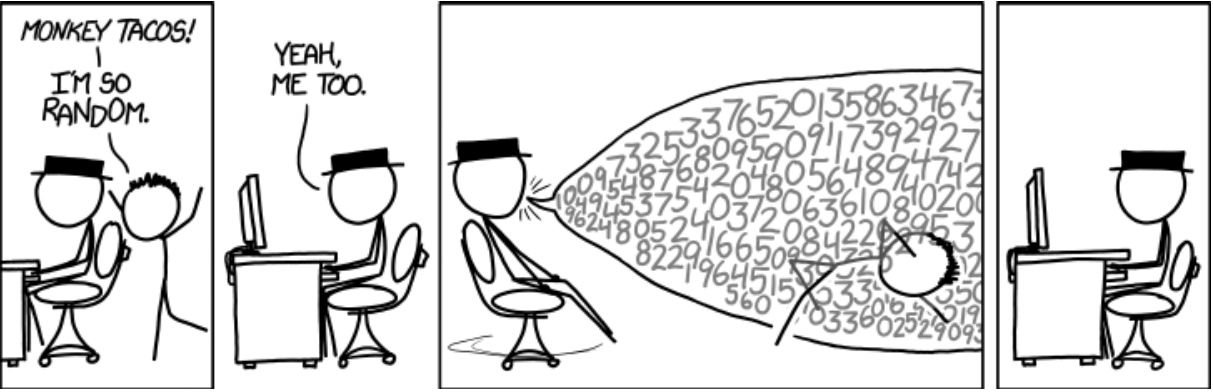
\includegraphics[width=1\linewidth]{images/im_so_random} 

}

\caption{Hauska kuva satunnaisuudesta.}\label{fig:random}
\end{figure}

Tässä luvussa pohdimme sattuman ja satunnaisuuden roolia tilastotieteessä ja tieteessä ylipäätään. Satunnaisuudella tarkoitetaan yleensä säännönmukaisuuden puuttumista ja ennustamattomuutta ja kenties juuri siksi sitä voidaan pitää yhtenä maailman vaikuttavammista ilmiöistä. Jokainen haluaisi tietää mitä tuleman pitää ja siksi sattuma on myös filosofisesti mielenkiintoinen: se vaikuttaa ja muokkaa niin meitä itseämme kuin ympäröivää maailmaa mitä merkityksellisimmin tavoin - joskus jopa vasten tahtoamme ja usein vailla täyttä ymmärtystämme!

Ihmisen oma kokemus on kuitenkin altis kaikenlaisille virhepäätelmille, joita kutsutaan myös kognitiivisiksi vinoumiksi. Haluamme löytää systematiikkaa ja tarkoitusta kaaoksesta sekä merkityksiä ja syy-seuraussuhteita sellaisista tapahtumista, jotka kuuluvat normaalivaihtelun piiriin. Tällaisissa tilanteissa usein tilastollinen tarkastelu paljastaakin ilmiön todellisen, alkuperäisestä kuvitelmasta poikkeavan luonteen. Osatakseen erottaa systemaattisen vaihtelun ja ymmärtääkseen oikeasti merkityksellisiä syy-seuraussuhteita, on välttämöntä ymmärtää satunnaisuutta. Tämä välttämättömyys pätee erityisesti tiedeyhteisön jäseniin, jotka pyrkivät tutkimaan ympäröivän maailman satunnaisia ilmiöitä. Tilastotiede perustuu satunnaisilmiöiden ja satunnaisen aineiston tutkimiseen, joten sen ymmärtäminen on keskeisessä roolissa tieteen ja maailman ymmärtämisessä.

\hypertarget{alaluku41}{%
\subsection{Satunnaisilmiöt ja satunnaismuuttujat tilastotieteessä}\label{alaluku41}}

\begin{itemize}
\tightlist
\item
  Edellisestä luvusta muistamme, että tilastotieteellisen tutkimuksen kohteena on aina jokin tilastoyksikköjen tutkimusmuuttujista koostuva havaintoaineisto, jonka pohjalta tehdään päätelmiä perusjoukosta/populaatiosta.
\item
  Nämä tilastolliset muuttujat tulkitaan satunnaisiksi, ja täten tilastollisen tutkimuksen tavoite on tutkia satunnaisilmiötä, joka on generoinut nämä havaitut eli toteutuneet arvot.

  \begin{itemize}
  \tightlist
  \item
    Yksi tilastotieteen olennainen tehtävä onkin kehittää \textbf{tilastollisia malleja}, joiden avulla satunnaisilmiöitä voidaan kuvata, selittää ja ennustaa.
  \item
    Tilastollisen mallin satunnaisten piirteiden kuvaus perustuu johonkin \textbf{todennäköisyysmalliin}.
  \end{itemize}
\end{itemize}

\begin{defblock}{}

\textbf{Satunnaisilmiö}

Reaalimaailman ilmiö on satunnaisilmiö, jos seuraavat ehdot pätevät:

\begin{itemize}
\tightlist
\item
  Ilmiöllä on useita erilaisia tulosvaihtoehtoja.
\item
  Sattuma määrää mikä tulosvaihtoehdoista toteutuu, eli yksittäistä tulosta ei voida tietää etukäteen.
\item
  Vaikka tulos vaihtelee ilmiön toistuessa satunnaisesti, käyttäytyy tulosvaihtoehtojen suhteellisten osuuksien jakauma tilastollisesti stabiilisti ilmiön toistokertojen lukumäärän kasvaessa.
\end{itemize}

\end{defblock}

\begin{itemize}
\tightlist
\item
  \textbf{Tilastollisella stabiiliudella} tarkoitetaan sitä, että on mahdollista arvioida kuinka \textbf{todennäköisiä} erilaiset tapahtumat, eli satunnaisilmiön tulosvaihtoehdot ovat.

  \begin{itemize}
  \tightlist
  \item
    Toisin sanoen satunnaisilmiön tulosvaihtoehtoihin on liityttävä säännönmukaisuutta, jonka on tultava esille ilmiön toistuessa.
  \end{itemize}
\end{itemize}

\begin{eblock}{}

\textbf{Esimerkkejä satunnaisilmiöistä} uudistettava\ldots{}

\begin{itemize}
\tightlist
\item
  Kvanttimekaniikan ja hiukkasfysiikan ilmiöt ovat perusluonteeltaan satunnaisia.
\item
  Luonnontieteellisiin mittauksiin liittyvien mittausvirheiden syntymekanismit ovat (ainakin osittain) satunnaisprosesseja.
\item
  Uhkapeleissä kuten arpajaisissa, lotossa, ruletissa, korttipeleissä ja noppapeleissä sattumalla on keskeinen rooli.
\item
  Perinnöllisyys noudattaa sattuman lakeja.
\item
  Eliöiden ominaisuuksien jakautuminen populaatiossa on satunnaista.
\item
  Ihmisten, ihmisryhmien ja ihmisten muodostamien organisaatioiden sosiaalisessa ja taloudellisessa käyttäytymisessä on monia satunnaisia elementtejä.
\item
  Teknisten prosessien tuloksien ominaisuudet jakautuvat satunnaisesti.
\end{itemize}

\end{eblock}

\hfill\break
\hfill\break

\textbf{Satunnaismuuttujat}

\begin{itemize}
\tightlist
\item
  Satunnaisilmiöitä koskevan tutkimuksen kohteena olevat tilastolliset muuttujat tulkitaan \textbf{satunnaismuuttujiksi} ja havainnot (havaintoarvot) voidaan näin ollen tulkita näiden satunnaismuuttujien realisoituneiksi arvoiksi. Satunnaismuuttuja siis kuvaa tarkasteltavan mitattavan ominaisuuden (satunnais)vaihtelua tutkimuksen kohteiden, eli tilastoyksiköiden joukossa.

  \begin{itemize}
  \tightlist
  \item
    Mitattavan ominaisuuden mahdolliset arvot määräävät satunnaismuuttujan luonteen. Yleisesti satunnaismuuttujat jaetaan kahteen luokkaan: \textbf{jatkuviin} ja \textbf{diskreetteihin}.
  \item
    Satunnaismuuttujan \textbf{todennäköisyysjakauma}, määrää erilaisten tulosvaihtoehtojen todennäköisyyden ja mahdollistaa täten tilastollisen analyysin ja päättelyn.

    \begin{itemize}
    \tightlist
    \item
      Satunnaisuus eroaa mielivaltaisesta prosessista siinä, että satunnaista ilmiötä voidaan kuvata jollakin \textbf{tilastollisella lailla} kun taas mielivaltaista prosessia ei.
    \end{itemize}
  \end{itemize}
\end{itemize}

\begin{defblock}{}

\textbf{Satunnaismuuttuja}

Satunnaismuuttuja (usein lyhyesti sm., englanniksi random variable, merkitään esim. \(Y\), ja kutsutaan ajoittain myös stokastiseksi muuttujaksi) on todennäköisyyslaskennan peruskäsite, jolla tarkoitetaan satunnaisilmiön määräämää lukua.

\begin{itemize}
\item
  Satunnaismuuttujan \(Y\) realisoituvaa arvoa \(y\) kutsutaan realisaatioksi tai toteumaksi.
\item
  Tilastollinen aineisto muodostuu useiden satunnaismuuttujien (tilastoyksiköiden tutkimusmuuttujien) realisoituneista arvoista.
\item
  Realisoituneiden arvojen vaihtelua tilastoyksiköiden välillä kutsutaan satunnaisvaihteluksi.\\
\end{itemize}

\end{defblock}

\begin{defblock}{}

\textbf{Jatkuvat ja diskreetit satunnaismuuttujat}

\begin{itemize}
\tightlist
\item
  Satunnaismuuttuja \(Y\) on jatkuva, jos se voi saada ylinumeroituvan määrän arvoja tai ts. minkä tahansa arvon joltain väliltä, kuten tyypillisesti minkä tahansa arvon joltain reaalilukuväliltä.
\item
  Satunnaismuuttuja \(Y\) on diskreetti, jos se voi saada vain joitain mahdollisia arvoja (vain yksittäisiä, äärellisen tai numeroituvasti äärettömän määrän, arvoja). Yksinkertaisimmillaan diskreetti satunnaismuuttuja \(Y\) on kaksiarvoinen (binäärinen), jolloin sen mahdollisia arvoja tyypillisesti merkitään \(y=0\) tai \(y=1\).
\end{itemize}

\end{defblock}

\begin{eblock}{}
\textbf{Esimerkki: satunnaismuuttuja}

Ihmisen pituutta voidaan pitää (ennen mittaukseen tulemista) satunnaismuuttujana \(Y\) ja lopullista pituutta täten pituuden realisaationa \(y\). Pituutta kohdellaan jatkuvana muuttujana senttimetreissä, mutta mikäli määritetään toteumaksi jonkin pituuden raja-arvon, esimerkiksi 170cm, ylittävä pituus, on kyseessä kaksiarvoinen (binäärinen) satunnaismuuttuja (pituus on joko yli tai alle 170 cm).

\end{eblock}

\begin{itemize}
\tightlist
\item
  Muuttujat voidaan luokitella myös \textbf{kvalitatiivisiin} ja \textbf{kvantitatiivisiin} muuttujiin.

  \begin{itemize}
  \tightlist
  \item
    Kvalitatiivisiin muuttujiin liittyy luokittelu- tai järjestysasteikko
  \item
    Kvantitatiivisiin muuttujiin välimatka- ja suhdeasteikko.
  \end{itemize}
\item
  Tilastolliset menetelmät perustuvat todennäköisyyslaskennan\footnote{Todennäköisyyslaskentaa käsitellään välillisesti tulevissa luvuissa mutta varsinaisesti tarkemmin 2. periodin kurssilla \href{https://opas.peppi.utu.fi/fi/opintojakso/TILM3553/1734?period=2022-2024}{TILM3553 Todennäköisyyslaskennan peruskurssi} ja (erityisesti sivuaineopiskelijoille) \href{https://opas.peppi.utu.fi/fi/opintojakso/TILM3568/3385?period=2022-2024}{TILM3568 Todennäköisyyslaskenta sivuaineopiskelijoille}.} tuloksiin ja tarjoavat keinon hallita satunnaisuuden aiheuttamaa epävarmuutta sekä tavan erottaa systemaattinen ja satunnainen vaihtelu, eli signaali ja kohina, toisistaan.
\item
  Tilastollisen aineiston \textbf{tilastollisella mallilla} tarkoitetaan täten niiden satunnaismuuttujien todennäköisyysjakaumaa, jonka ajatellaan generoineen havainnot.

  \begin{itemize}
  \tightlist
  \item
    Yksinkertaisimmillaan esimerkiksi yksinkertaiseen satunnaisotantaan takaisinpanolla perustuva satunnaismalli (palaamme tähän otantaa käsittelevässä luvussa \ref{luku5}).
  \item
    Satunnaisuus perustuu siihen, että satunnaismuuttujien toteutuvat arvot (ja niistä lasketut tunnusluvut kuten keskiarvo) vaihtelevat satunnaisesti otoksesta toiseen.
  \end{itemize}
\item
  Todennäköisyyslaskennan tehtävä on tuottaa \textbf{matemaattisia ja tilastollisia malleja} satunnaisilmiöissä havaittavalle tilastolliselle stabiliteetille.
\end{itemize}

\hypertarget{alaluku42}{%
\subsection{Tilastotieteen suhde satunnaisuuteen ja todennäköisyyksiin}\label{alaluku42}}

\begin{itemize}
\tightlist
\item
  Tilastotieteessä \textbf{tutkimusaineiston keräämistä} voidaan pitää hyvänä esimerkkinä satunnaisilmiöstä.

  \begin{itemize}
  \tightlist
  \item
    Voimme ajatella, että tilastollisen tutkimuksen kohteet on aina valittu arpomalla.
  \item
    Arvonta on mainio esimerkki satunnaisilmiöstä, sillä siihen liittyy aina ennustamattomuutta: vaikka yksittäisen arvonnan tulosta ei voi tietää etukäteen, noudattaa se kuitenkin todennäköisyyden lakeja.
  \item
    Koska arvonnan tulos vaihtelee satunnaisesti arvontakerrasta toiseen, myös tutkimuksen kohteita kuvaavat tiedot vaihtelevat satunnaisesti arvontakerrasta toiseen.
  \item
    Tutkimuksen kohteita kuvaavien tietojen käyttäytymisessä havaitaan kuitenkin arvontaa toistettaessa juuri sitä säännönmukaisuutta, jota kutsutaan tilastolliseksi stabiliteetiksi. \textbf{Tämä säännönmukaisuus on tilastollisen tutkimuksen kohde.}
  \end{itemize}
\item
  Esimerkkejä tilastollisten aineistojen keräämisen menetelmistä, jotka perustuvat arvontaan:

  \begin{itemize}
  \tightlist
  \item
    \textbf{Satunnaistetut kokeet}: Kokeellisessa tutkimuksessa tavoitteena on vertailla erilaisten käsittelyiden vaikutuksia kokeen kohteisiin. Erilaisten virhelähteiden kontrolloimiseksi käsittelyt on syytä arpoa kohteille.
  \item
    \textbf{Satunnaisotanta}: Otannalla\footnote{Erityisesti erilaisten otantamenetelmien yhteydessä, joita tarkastellaan tarkemmin luvussa \ref{luku5}.} tarkoitetaan laveasti tutkimusaineistojen keräämisen menetelmiä. Erilaisten virhelähteiden kontrolloimiseksi tutkimuksen kohteet on syytä valita arpomalla. (Ks. Luku \ref{luku5})
  \end{itemize}
\item
  Kerätyn (tai havaitun) aineiston pohjalta tehdään päätelmiä sen generoineesta satunnaisilmiöstä esimerkiksi testaamalla erilaisia siihen liittyviä hypoteeseja.

  \begin{itemize}
  \tightlist
  \item
    Tilastotiede voidaan jakaa kahteen suureen paradigmaan sen mukaan, miten tilastolliseen päättelyyn, ml. hypoteeseihin ja niiden testaamiseen, suhtaudutaan. Näitä ovat \textbf{klassinen eli frekventistinen tilastotiede} sekä \textbf{Bayesilainen tilastotiede}. Tarkastellaan seuraavaksi minkälaisia eroja ja yhtäläisyyksiä näiden koulukuntien välillä on.
  \end{itemize}
\end{itemize}

\hfill\break
\hfill\break

\textbf{Frekventistinen tilastotiede}

\begin{itemize}
\item
  Klassisessa eli frekventistisessä tilastotieteessä ajatellaan että hypoteesien testaaminen tulee perustua yksinomaan havaittuun aineistoon ja siihen liitettävään tilastolliseen malliin.
\item
  Nimi ``frekventistinen'' juontuu siitä, että tämä todennäköisyysjakauma määrittää satunnaismuuttujan mahdollisten arvojen todennäköisyydeksi niiden suhteellisen osuuden äärettömästä määrästä realisaatioita, ts. niiden suhteellisen frekvenssin.
\item
  Klassisessa tilastotieteessä havaittuun aineistoon \emph{sovitetaan} sitä kuvaavaan todennäköisyysjakaumaan perustuva tilastollinen malli, joka vastaa saatua aineistoa parhaiten.

  \begin{itemize}
  \tightlist
  \item
    Tämä tilastollinen malli perustuu nk. \textbf{uskottavuusfunktioon}, joka on \emph{aineiston} sekä yhden tai useamman \emph{parametrin} funktio ja joka saavuttaa suurimman arvonsa nk. ``suurimman uskottavuuden pisteessä''.
  \item
    Uskottavuusfunktio kertoo kuinka todennäköisenä havaittua aineistoa voidaan pitää, mikäli sen oletetaan olevan peräisin vastaavasta mallista jollain parametriarvolla. Täten ne parametriarvot, joilla uskottavuusfunktion arvo maksimoituu, kuvaavat aineiston generoimaa prosessia parhaiten, annettuna malli- eli jakaumaoletus.
  \item
    Uskottavuusfunktioista, tilastollisten mallien estimoinnnista ja parametreista lisää seuraavassa alaluvussa sekä luvussa \ref{luku6}.
  \end{itemize}
\item
  Perusjoukkoa koskevia hypoteeseja testataan tämän tilastollisen mallin avulla: havaittu aineisto määrittää uskottavuusfunktion perusteella sellaiset hypoteesit, jotka jäävät joko voimaan tai tulevat hylätyiksi.
\item
  Klassisessa tilastotieteessä hypoteesien testaus perustuu siis vain aineistoon eli tilastollinen päättely on induktiivista: aineiston avulla otosta koskeva päätelmä voidaan yleistää koskemaan perusjoukkoa.

  \begin{itemize}
  \tightlist
  \item
    Toki kaikki päättely on alisteista tehdyille oletuksille koskien käytettävää tilastollista mallia.
  \end{itemize}
\end{itemize}

\hfill\break
\hfill\break

\textbf{Bayesilainen tilastotiede}

\begin{itemize}
\tightlist
\item
  Bayesilainen tilastotiede on tilastotieteen toinen suuri paradigma ja on saanut nimensä englantilaiselta harrastelijamatemaatikko ja presbyteeripappi \href{https://fi.wikipedia.org/wiki/Bayesil\%C3\%A4inen_tilastotiede}{Thomas Bayesilta}, jota pidetään Bayesilaisen tilastotieteen isänä.
\item
  Bayesilainen tilastotiede ulottaa todennäköisyyskäsityksen, eli tn-jakauman, myös aineistoa koskevien hypoteesien puolelle: kuinka todennäköisenä jotain hypoteesia voidaan pitää jo ennen tutkimusaineiston keräämistä?

  \begin{itemize}
  \tightlist
  \item
    Myös Bayesilaisessa tilastotieteessä hyödynnetään uskottavuusfunktiota, mutta hypoteesien testaus ei perustu niinkään frekventistiseen ajatukseen todennäköisyyksistä suhteellisina osuuksina äärettömässä sarjassa.
  \item
    Bayesilaiset perustavat sen sijaan hypoteesien testaamisen tutkimuskysymystä koskevien ennakkokäsitysten päivittämiselle sen jälkeen, kun aineiston on havaittu.
  \item
    Nämä ennakkokäsitykset voidaan kuvata todennäköisyysjakaumana, priorijakaumana, jota päivitetään ns. posteriorijakaumaksi kun aineisto havaitaan. Näin päättely perustuu priorijakauman ja aineiston uskottavuusfunktion väliselle kompromissille!
  \end{itemize}
\item
  Ajatusta ennakkokäsityksistä todennäköisyyksinä käytetään niin Bayesilaisen tilastotieteen kritiikkinä kuin puolustuksena.

  \begin{itemize}
  \tightlist
  \item
    Lopulta olemme kaikki Bayesilaisia: jokaisella on sisäisiä ennakkokäsityksiään, myös tutkijoilla! Nämä ennakkokäsitykset voivat perustua esimerkiksi aiempaan tutkittuun tietoon, mutta myös uskomuksiin.
  \item
    Prioritiedon hyödyntäminen tilastollisessa tutkimuksessa on usein perusteltua.
  \item
    Bayesilaista tilastotiedettä tarkastellaan tarkemmin esimerkiksi kursseilla \href{https://opas.peppi.utu.fi/fi/opintojakso/TILM3577/6969}{TILM3577 Bayes-päättely} sekä \href{https://opas.peppi.utu.fi/fi/opintojakso/TILM3601/21033}{TILM3601 Bayes-laskenta}.
  \end{itemize}
\end{itemize}

\hypertarget{alaluku43}{%
\subsection{Tilastolliset mallit, jakaumat ja parametrit}\label{alaluku43}}

\begin{itemize}
\tightlist
\item
  Tilastolliset mallit perustuvat satunnaismuuttujan mahdollisten tulosvaihtoehtojen todennäköisyyksiä kuvaavalle \textbf{todennäköisyysjakaumalle}, joka määrää millä todennäköisyydellä satunnaismuuttuja saa erilaisia arvoja.
\item
  Toisaalta ajoittain tietyn suureen/ilmiön mallinnuksessa voidaan perustellusti käyttää molempiin luokkiin kuuluvien satunnaismuuttuja- ja tilastollisen mallityypin vaihtoehtoja.

  \begin{itemize}
  \tightlist
  \item
    Esimerkki: Esimerkiksi COVID19-tartuntatapausten lukumäärä Suomessa on periaatteessa diskreetti satunnaismuuttuja, joka saa yksittäisen (kokonaisluku)arvon joka kuukausi, mutta käytännössä lukumäärät ovat tässä tapauksessa sen verran suuria, että niitä (saatetaan) mallintaa jatkuva-arvoisena muuttujana.
  \item
    Vastaavasti esimerkiksi potilaan jonotusaika päivystyksessä voi periaatteessa saada minkä tahansa arvon tietyltä reaalilukuväliltä (tällöin käytettäisiin jatkuviin sm:jiin perustuvia tilastollisia menetelmiä).
  \end{itemize}
\item
  Satunnaismuuttujan mahdolliset arvot, ja täten todennäköisyysjakauma, määräävät myös käytettävän tilastollisen mallin.

  \begin{itemize}
  \tightlist
  \item
    \textbf{Diskreetin satunnaismuuttujan} jakauma voidaan usein esittää taulukkomuodossa. Eri arvojen todennäköisyydet muodostavat kyseisen satunnaismuuttujan todennäköisyysjakauman (\textbf{pistetodennäköisyysfunktion}), jota voidaan havainnollistaa esimerkiksi pylväsdiagrammilla.
  \item
    Jatkuvan satunnaismuuttujan \(Y\) arvot muodostavat jonkin reaaliakselin välin, joka sisältää äärettömän määrän lukuja. Tämän vuoksi jatkuvan satunnaismuuttujan jakauman esittäminen taulukossa ei ole luontevaa, vaan jakauma esitetään yleensä satunnaismuuttujan \textbf{tiheysfunktion} avulla.

    \begin{itemize}
    \tightlist
    \item
      Pistetodennäköisyys- ja tiheysfunktio siis määräävät satunnaismuuttujan mahdollisille arvoille todennäköisyydet väliltä \([0,1]\) ja näin voidaan arvioida havaitun aineiston uskottavuutta ja testata siihen liitettäviä hypoteeseja suhteessa estimoituun suuriman uskottavuuden estimaattiin.
    \end{itemize}
  \end{itemize}
\item
  Tilastolliset mallit approksimoivat ``todellista'' aineiston generoinutta ilmiötä. Tilastolliset mallit riippuvat \textbf{parametreista} ja keskeinen oletus erityisesti klassisessa tilastotieteessä on, että aineiston generoinutta satunnaisilmiötä kuvaa jokin vakioinen mutta tuntematon parametriarvo (tai niiden joukko).
\end{itemize}

\begin{figure}

{\centering 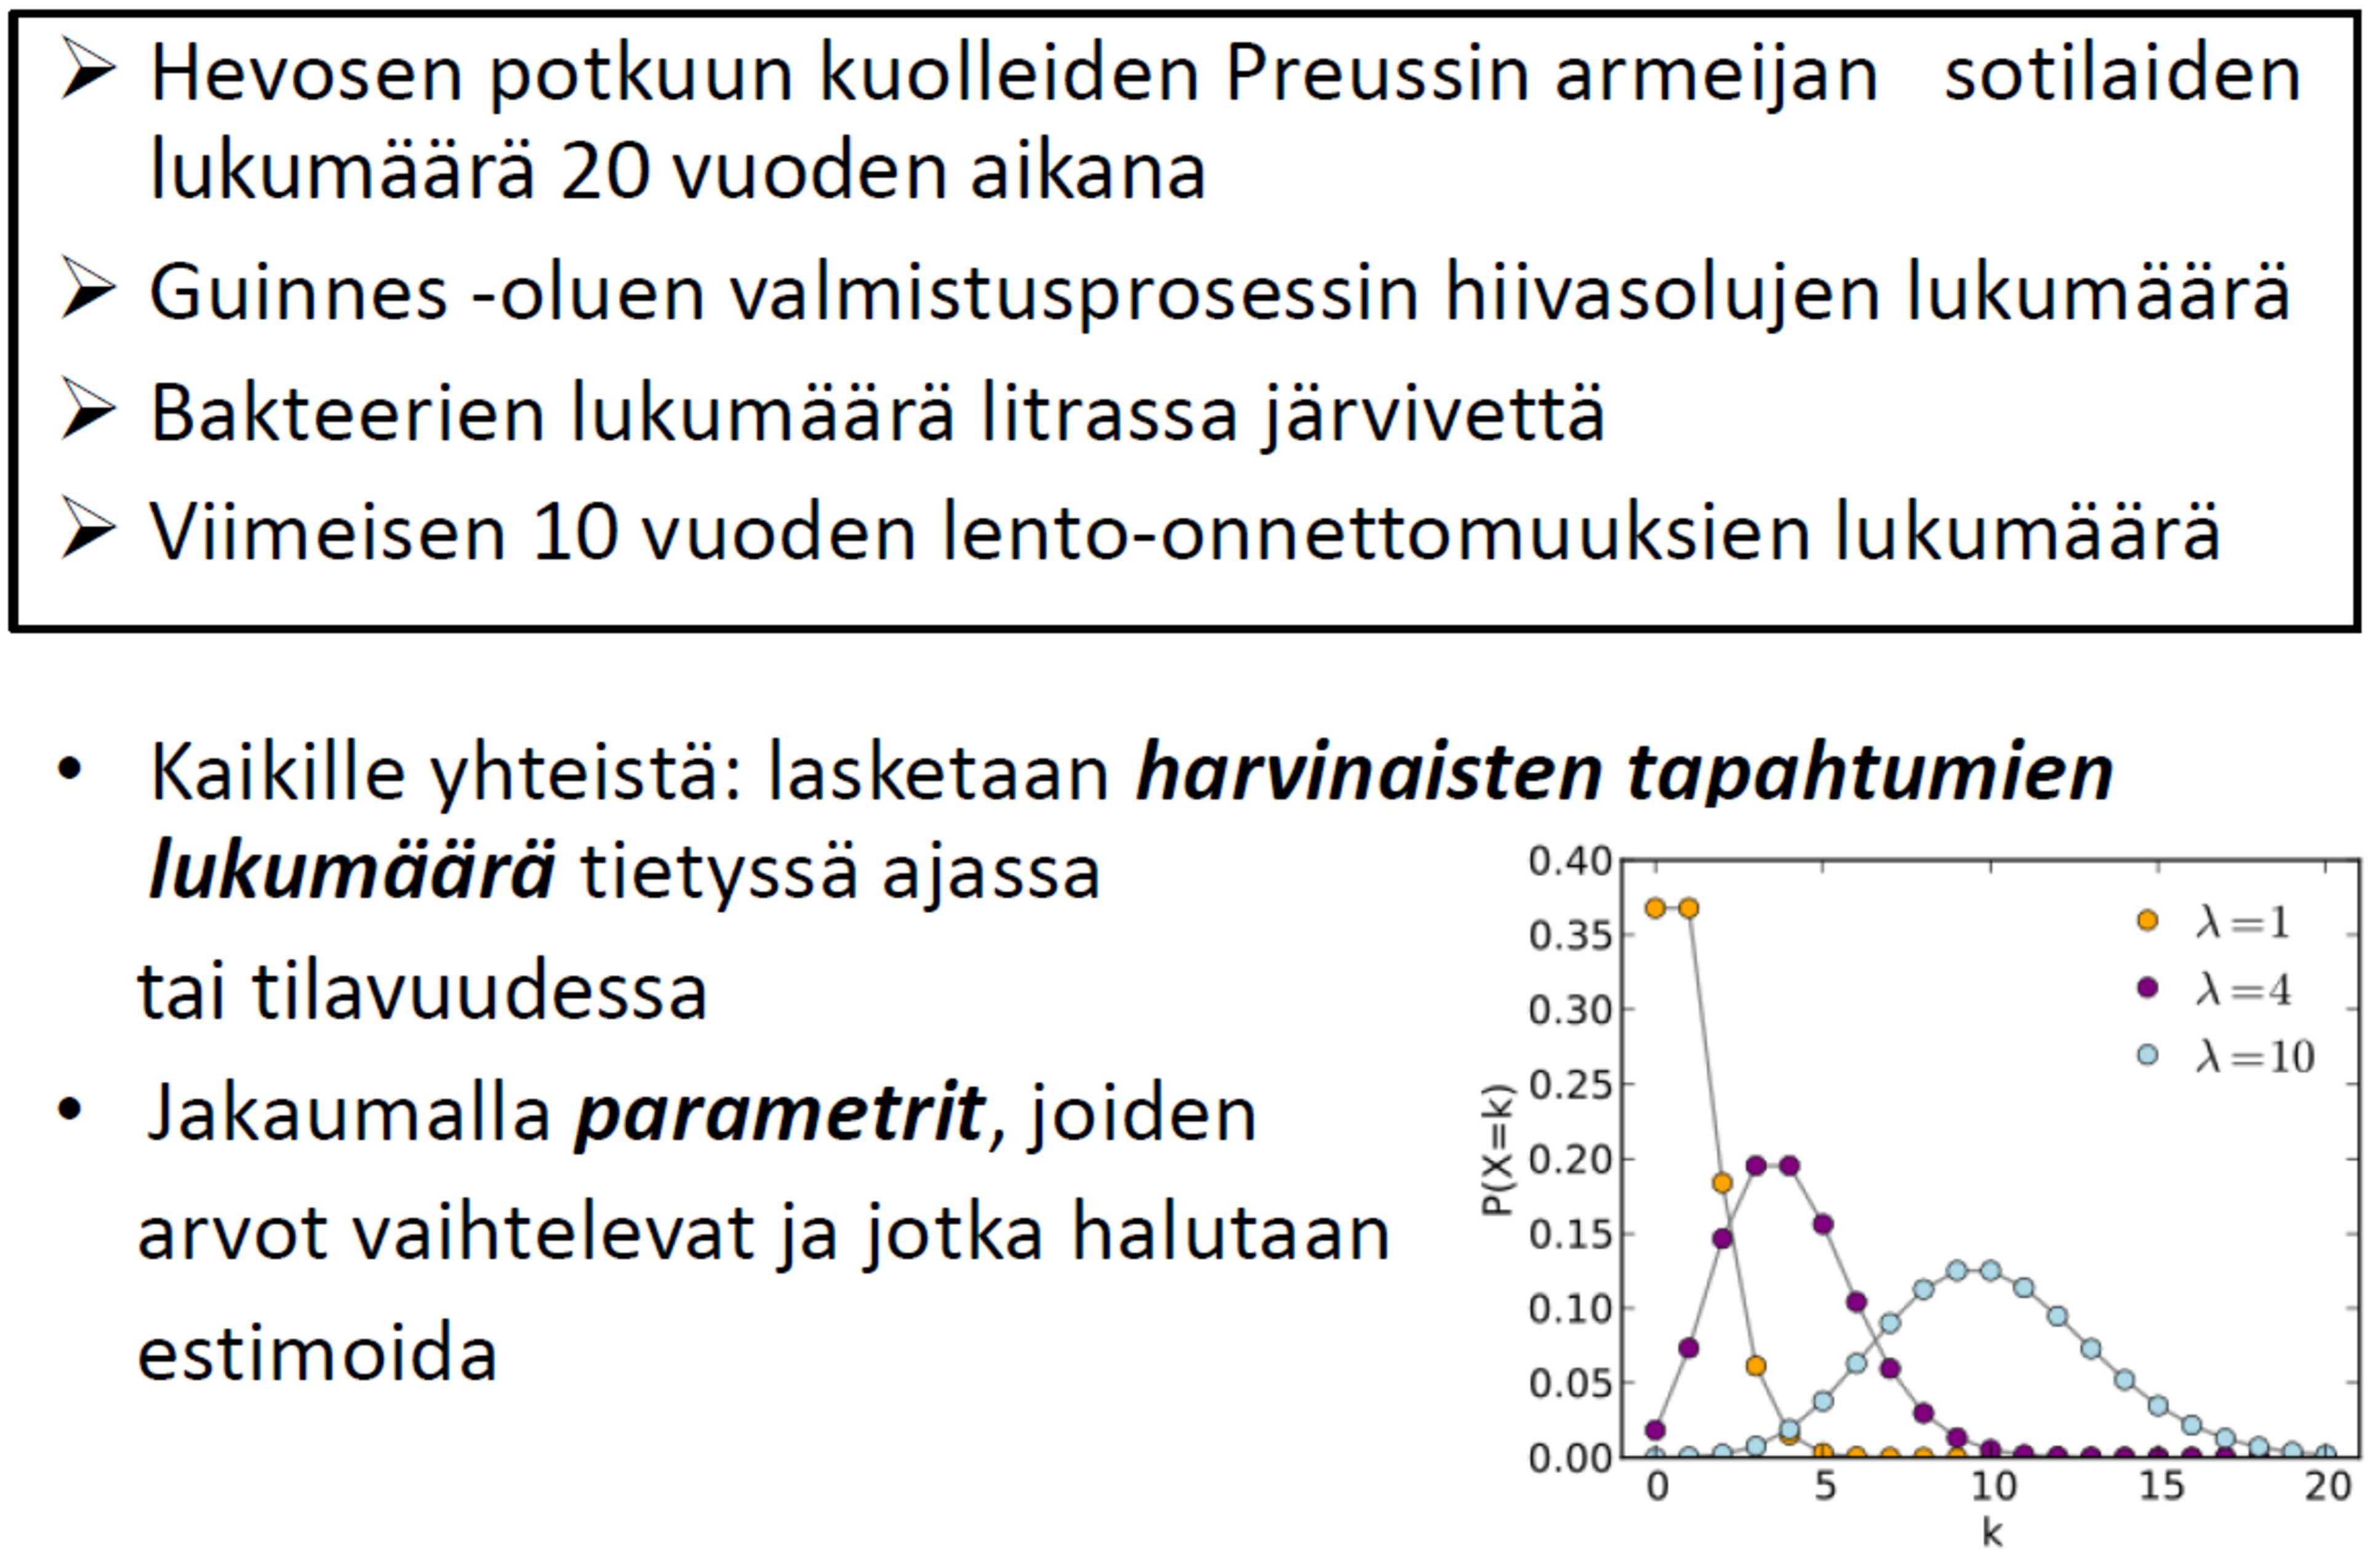
\includegraphics[width=1\linewidth]{images/poisson} 

}

\caption{Esimerkki: Poisson-jakauman sovelluskohteita ja sen pistetodennäköisyysfunktio eri parametrin arvoilla. Poisson-jakaumaa esitellään tarkemmin alaluvussa 4.5.}\label{fig:poisson}
\end{figure}

\hfill\break
\hfill\break

\textbf{Parametrien estimointi ja niiden testaus}

\begin{itemize}
\tightlist
\item
  Satunnaisilmiötä kuvaava tilastollinen malli perustuu siis johonkin parametriseen todennäköisyysjakaumaan, joka yhdessä havaintojen kanssa määrittää uskottavuusfunktion.

  \begin{itemize}
  \tightlist
  \item
    Aineistoa kuvaavan tilastollisen mallin uskottavuus pyritään maksimoimaan, mikä tarkoittaa valitun todennäköisyysjakauman sovittamista havaintoaineistoon mahdollisimman hyvin.
  \item
    Tässä nk. ``suurimman uskottavuuden estimoinnissa'' aineiston generoiman (oletetun) todennäköisyysjakauman parametriarvot \textbf{estimoidaan} (eli arvioidaan) käytettävän otoksen/aineiston avulla.
  \item
    Perusjoukkoa parhaiten kuvaavan (eli ``aineiston generoineen'') parametrin arvo pyritään siis estimoimaan aineiston perusteella.
  \end{itemize}
\item
  Parametrien estimoinnin lisäksi usein \textbf{testataan} parametreja koskevia oletuksia (eli hypoteeseja).
\item
  Estimointi ja testaus ovat tilastolliseen tutkimukseen liittyvän \textbf{tilastollisen päättelyn} keskeisiä välineitä, joiden avulla tutkittavasta ilmiöstä pyritään tekemään johtopäätöksiä siitä kerätyn havaintoaineiston perusteella.

  \begin{itemize}
  \tightlist
  \item
    Estimoitujen parametrien testaus voi vastata esimerkiksi seuraavanlaisiin kysymyksiin:

    \begin{itemize}
    \tightlist
    \item
      Onko suomalaisten miesten keskipituus 180cm?
    \item
      Vaikuttaako yliopistokoulutus tulevaisuuden ansioihin?
    \item
      Auttaako tietty lääkeaine jonkin sairauden hoidossa?
    \item
      Voiko osakemarkkinoiden tuottoja ennustaa?
    \end{itemize}
  \end{itemize}
\item
  Parametrien testaus on osa tilastollista päättelyä, johon palataan tarkemmin luvussa \ref{luku6}
\end{itemize}

\hypertarget{alaluku44}{%
\subsection{Odotusarvo ja varianssi}\label{alaluku44}}

\begin{itemize}
\tightlist
\item
  Satunnaismuuttujan todennäköisyysjakauman tietoa voidaan tiivistää tunnuslukuihin, joista keskeisimpiä ovat \textbf{odotusarvo}, \textbf{varianssi} ja \textbf{keskihajonta}.
\end{itemize}

\begin{defblock}{}

\textbf{Odotusarvo}

Satunnaismuuttujan \(Y\) odotusarvo \(\text{E}(Y)\) kuvaa satunnaismuuttujan odotettavissa olevaa arvoa.

\begin{itemize}
\tightlist
\item
  Muodostamalla satunnaiskokeen tulosten \textbf{painotettu keskiarvo}, jossa kunkin tuloksen painona on vastaavan tapauksen todennäköisyys, niin saatua arvoa sanotaan odotusarvoksi \(\text{E}(Y)\).
\item
  Odotusarvo kuvaa jakauman painopistettä.
\item
  Merkinnän \(\text{E}(Y)\) käyttö juontaa juurensa englannin kielen sanoihin ``odotus'', expectation, ja `odotusarvo', expected value.
\end{itemize}

\end{defblock}

\begin{eblock}{}
\textbf{Esimerkki: Odotusarvo}

tähän joku esimerkki tosiaan.

\end{eblock}

\hfill\break
\hfill\break

\begin{itemize}
\tightlist
\item
  Odotusarvon lisäksi kiinnostuksen kohteena on usein jakauman keskittyneisyys (hajaantuneisuus). Ts. kun halutaan puolestaan kuvata satunnaismuuttujan arvojen vaihtelua, tutkitaan todennäköisyysjakauman \textbf{varianssia} ja \textbf{keskihajontaa}.
\end{itemize}

\begin{defblock}{}
\textbf{Varianssi}

Satunnaismuuttujan \(Y\) hajontaa voidaan mitata varianssilla
\[
\mathrm{Var}(Y) = \text{E}\Big[\Big(Y-\text{E}(Y)\Big)^2\Big],
\]
tai sen neliöjuuren eli \textbf{keskihajonnan} avulla
\[
\text{D}(Y) = \sqrt{\mathrm{Var}(Y)}.
\]
- Mitä lähempänä nollaa keskihajonta ja varianssi ovat, sitä todennäköisempää on, että satunnaismuuttujan arvo on lähellä odotusarvoa.
- Merkintöjen \(\mathrm{Var}(Y)\) ja \(\text{D}(Y)\) taustalla on englannin kielen sanat variance (varianssi) ja deviation, joka
tarkoittaa poikkeamaa, hajontaa.

\end{defblock}

\begin{itemize}
\tightlist
\item
  Odotusarvon ja varianssin (keskihajonnan) tavanomaiset estimaattorit ovat otoskeskiarvo ja otosvarianssi (otoshajonta), joihin palataan vielä myöhemmin.
\end{itemize}

\hypertarget{alaluku45}{%
\subsection{Joitain jakaumia}\label{alaluku45}}

Tarkastellaan seuraavassa muutamia keskeisiä tilastollisia jakaumia. Esittelemme ensin keskeisintä jatkuvien satunnaismuuttujien jakaumaa, normaalijakaumaa, ennen muutamien diskreettien satunnaismuuttujien jakaumia.

\hypertarget{normaalijakauma}{%
\subsubsection{Normaalijakauma}\label{normaalijakauma}}

\begin{itemize}
\item
  Jos satunnaismuuttuja \(Y\) noudattaa \textbf{normaalijakaumaa} odotusarvolla \(\text{E}(Y)= \mu\) ja varianssilla \(\mathrm{Var}(Y) = \sigma^2\), niin tällöin merkitään \(Y \thicksim \text{N}(\mu, \sigma^2)\).
\item
  \(Y\):n tiheysfunktio on muotoa (ks. kuva alla)
  \[
  f(y; \mu, \sigma^2) = \frac{1}{\sqrt{2 \pi \sigma^2}} \, e^{-\frac{1}{2} \Big(\frac{y- \mu}{\sigma} \Big)^2}, 
  \]
  jossa \(e\) viittaa Neperin lukuun \(e \approx 2,71828\)

  \begin{itemize}
  \tightlist
  \item
    Ylläoleva tf. määrittelee parven normaalijakaumia kun parametreille (vakioille) \(\mu\) ja \(\sigma^2\) annetaan erilaisia arvoja. Nämä kaksi parametria määräävät normaalijakauman tarkemman muodon.
  \end{itemize}
\end{itemize}

\begin{figure}

{\centering 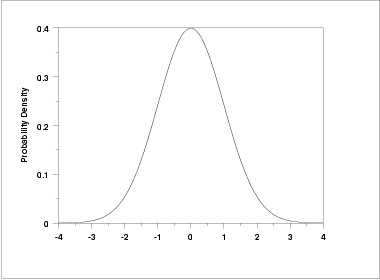
\includegraphics[width=1\linewidth]{images/normpdf} 

}

\caption{Normaalijakauma}\label{fig:normpdf}
\end{figure}

\begin{eblock}{}

\textbf{Esimerkki: Miesten pituus}

\begin{itemize}
\tightlist
\item
  Tutkitaan miesten pituutta hyvin määritellyssä joukossa, kuten varusmiespalvelusta tiettynä vuonna suorittavien joukossa.

  \begin{itemize}
  \tightlist
  \item
    Pituus on ominaisuus, jonka voidaan nähdä määräytyvän monista perintö- ja ympäristötekijöistä. Pituutta voidaan siis pitää satunnaismuuttujana.
  \item
    Oletetaan, että pituus noudattaa normaalijakaumaa. Näin ollen sm. \(Y\) on valitun miehen pituus ja \(Y \thicksim \text{N}(\mu, \sigma^2)\).
  \end{itemize}
\item
  Tuntemattomien parametrien \(\mu\) ja \(\sigma^2\) tulkinta:

  \begin{itemize}
  \tightlist
  \item
    Odotusarvo \(\mu = \text{E}(Y)\) on satunnaisesti valitun miehen pituuden odotettavissa oleva arvo.
  \item
    Varianssi \(\sigma^2 = \mathrm{Var}(Y) = \text{E} \Big[\Big(Y- \mu \Big)^2 \Big]\) kuvaa valitun miehen pituuden odotusarvostaan määrätyn poikkeaman (keskihajonnan) neliön odotettavissa olevaa arvoa (kuvaten ts. pituuksien jakauman keskittyneisyyttä/hajaantuneisuutta pituuksien odotusarvon ympärillä).
  \end{itemize}
\end{itemize}

\end{eblock}

\hfill\break
\hfill\break

\hypertarget{bernoulli--binomi--ja-poisson-jakauma}{%
\subsubsection{Bernoulli-, binomi- ja Poisson-jakauma}\label{bernoulli--binomi--ja-poisson-jakauma}}

\begin{itemize}
\tightlist
\item
  \textbf{Bernoulli-jakauma} on todennäköisyysjakauma, jossa satunnaismuuttujalla \(Y\) on kaksi mahdollista tulosvaihtoehtoa \(Y=1\) tai \(Y=0\).

  \begin{itemize}
  \tightlist
  \item
    Yleensä \(Y=0\) tarkoittaa, että jokin tapahtuma ei tapahdu ja \(Y=1\) että tapahtuu.
  \item
    Todennäköisyys tapahtumalle \(Y=1\) on \(\text{P}(Y=1)=p\) ja vastaavasti vastatodennäköisyys \(\text{P}(Y=0)=1-p\).
  \item
    Bernoulli-jakaumaa merkitään \(Y \thicksim B(p)\), jossa siis \(0 < p < 1\).
  \item
    Bernoulli-jakauman \textbf{pistetodennäköisyysfunktio} on muotoa
  \end{itemize}
\end{itemize}

\[
f(y; p) = \text{P}(Y=y) = p^y (1-p)^{(1-y)},
\]
jossa \(y\) on sm:n \(Y\) realisaatio (havaittu arvo) ja parametri \(p\) on tuntematon (voidaan estimoida otoksen avulla).

\begin{itemize}
\tightlist
\item
  Bernoulli-jakauman odotusarvo \(\text{E}(Y)=p\) ja varianssi \(\mathrm{Var}(Y)=p (1-p)\).
\end{itemize}

\hfill\break
\hfill\break

\begin{itemize}
\tightlist
\item
  \textbf{Binomijakauma}

  \begin{itemize}
  \tightlist
  \item
    Olkoon \(Y_1, \ldots, Y_n\) riippumattomia satunnaismuuttujia ja \(Y_i \thicksim B(p), \, i=1,\ldots,n\).
  \item
    Jos \(X = Y_1 + Y_2 + \ldots + Y_n\), niin \(X \thicksim \mathrm{Bin}(n,p)\). Ts. sm. \(X\) noudattaa \textbf{binomijakaumaa} parametrein \(n\) ja \(p\).
  \item
    Pistetodennäköisyysfunktio:
  \end{itemize}
\end{itemize}

\[
\text{P}(X=k) = \binom nk p^k (1-p)^{(n-k)}.
\]

\begin{itemize}
\tightlist
\item
  Jakauman odotusarvo \(\text{E}(X)=np\) ja varianssi \(\mathrm{Var}(X) = n p (1-p)\).
\item
  Binomijakaumalla kyetään vastaamaan mm. kysymykseen millä todennäköisyydellä \(n\):n kokoisessa otoksessa tapahtuu \(k\) onnistumista.
\end{itemize}

\begin{eblock}{}
\textbf{Esimerkki: Miesten lukumäärä Saksin osavaltion perheissä 1876--1885}\footnote{Ks. tarkemmin esimerkki 3.2 kirjassa (s. 67-68) Friendly, M., ja D. Meyer (2015). \emph{Discrete Data Analysis with R. Visualization and Modeling Techniques for Categorical and Count Data.} Chapman \& Hall/CRC.}

Vuosien 1876--1885 aikana Saksin osavaltiossa rekisteröitiin yli neljä miljoonaa syntynyttä lasta. Tällöin vanhempien tuli ilmoittaa lapsen sukupuoli (mies tai nainen) heidän syntymätodistuksessaan. Myöhemmässä tutkimuksessa tutkittiin tarkemmin 6115 perhettä, joissa asui 12 lasta ja tarkemmin miesten (poikien) lukumäärää näissä perheissä.

Seuraavassa taulukossa taulukoidaan miesten (poikien) lukumäärät näissä 12 lapseen perheissä:

\textbar Miesten lkm. (\(k\))\textbar0\textbar1\textbar2\textbar3\textbar4\textbar5\textbar6\textbar7\textbar8\textbar9\textbar10\textbar11\textbar12\textbar{}
\textbar Perheiden lkm. (\(n_k\))\textbar3\textbar24\textbar104\textbar286\textbar670\textbar1033\textbar1343\textbar1112\textbar829\textbar478\textbar181\textbar45\textbar7\textbar{}

Tarkasteltava jakauma esitetään vielä erikseen allaolevassa kuviossa.

Tässä tilantessa mielenkiinnon kohteena saattaisi olla hypoteesi, jonka mukaan pojan (miehen) syntymätodennäköisyys \(\text{P}(\mathrm{mies}) = p\) on \(p=0.5\).

\end{eblock}

\hfill\break
\hfill\break

\textbf{Poisson-jakauma}

\begin{itemize}
\item
  Jos satunnaismuuttuja \(Y\) on Poisson-jakautunut, merkitään \(Y \thicksim P(\lambda)\), jossa parametri \(\lambda > 0\) on Poisson-jakauman parametri, jota kutsutaan myös ajoittain intensiteettiparametriksi.
\item
  Poisson-jakaumaa voidaan käyttää tilanteissa, joissa sm. \(Y\) on jokin lukumäärä ja sen pistetodennäköisyysfunktio on muotoa
  \[
  \text{P}(Y=k) = \frac{e^{-\lambda} \lambda^k}{k!}
  \]
\item
  Odotusarvo ja varianssi ovat Poisson-jakauman tapauksessa samat: \(\text{E}(Y) = \mathrm{Var}(Y) = \lambda\).
\end{itemize}

\begin{eblock}{}
\textbf{Esimerkki: Poisson-jakauma}

Tarkastellaan Englannin Valioliigakauden 1995--1996 otteluissa tehtyjä maalimääriä. Valioliiga (The F.A. Premier League) on korkein Englannin jalkapalloliigan sarjataso, jossa ensi kerran juuri kaudella 1995-1996 20 joukkuetta (aiemmin Valioliigan perustamisen kauden 1992--1993 alussa 22 joukkuetta) pelasivat keskenään kerran toisiaan vastaan koti- ja vieraskentällä. Otteluita oli siis yhteensä 380.

Tämä esimerkki perustuu edellä mainittuun Friendlyn ja Meyerin (2015) kirjan esimerkkiin 3.9 (s. 78-79), joka vastaavasti perustuu Alan J. Leen (1997) artikkeliin\footnote{Alan J. Lee (1997). Modeling Scores in the Premier League: Is Manchester United Really the Best? \emph{Chance} 10(1), 15-19.}, jonka esittämään kysymykseen (hypoteesiin) vastaus on tietenkin ilmeinen! Näin ollen seuraavassa tarkastellaankin kotijoukkueiden ja vierasjoukkueiden maalintekointensiteettiä Poisson-jakaumaan perustuen. Seuraavassa emme siis pyri mallintamaan tietyn spesifin ottelun lopputulosta vaan tarkastelemme ``keskimääräisen'' kotijoukkueen ja vierasjoukkueen ``edustavaa'' ottelua.

Seuraava taulukko raportoi tehtyjen maalimäärien jakaumat pelatuissa 380 ottelussa. Neljän tai yli neljän maalin tapaukset kirjataan 4+:nä maalina. Ts. esim. kys. kauden lopputulokset \emph{Blackburn Rovers}- \emph{Nottingham Forest} 7-0 ja \emph{Bolton Wanderers} - \emph{Manchester United} 0-6 tulevat aineistoon tuloksina 4+ vs.~0 ja 0 vs.~4+.

\begin{center}
 \begin{tabular}{c|ccccc|c}
\hline \hline
Kotij. maalien & \multicolumn{5}{c}{Vierasj. maalien lkm.} & Yht. \\
lkm. & 0 & 1 & 2 & 3 & 4+ &  \\
\hline
0 & 27 & 29 & 10 & 8 & 2 & 76 \\
1 & 59 & 53 & 14 & 12 & 4 & 142 \\
2 & 28 & 32 & 14 & 12 & 4 & 90 \\
3 & 19 & 14 & 7 & 4 & 1 & 45 \\
4+ & 7 & 8 & 10 & 2 & 0 & 27 \\
\hline
Yht. & 140 & 136 & 55 & 38 & 11 & 380 \\
    \hline \hline
\end{tabular}
\end{center}

Olettamalla, että koti- ja vierasjoukkueen todennäköisyys tehdä maali ottelun aikana on vakio, niin tällöin koti- ja vierasjoukkueen ottelun aikana tekemien maalien lukumäärää (ilman edellä käytettyä maalimäärien ``katkaisua'' neljään) voidaan melko hyvin approksimoida oletuksella, että nämä lukumäärät ovat Poisson-jakautuneita. Ts. \(Y^H_i \thicksim P(\lambda_H)\) on sm., joka kuvaa \(i\):n ottelun kotijoukkueen tekemien maalien lukumäärää ja intensiteettiparametrin \(\lambda_H\) arvon määrittäminen kuuluu tilastollisen päättelyn ja erityisesti estimointiteorian piiriin. Vastaavasti vierasjoukkueen maalimäärät: \(Y^A_i \thicksim P(\lambda_A)\).

Osoittautuu, että parametreille \(\lambda_H\) ja \(\lambda_A\) saatavat estimaatit ovat \(\lambda_H = 1,49\) ja \(\lambda_A = 1,06\) ja ne vastaavat tässä yksinkertaistetussa tilanteessa koti- ja vierasjoukkueen keskimääräisiä maalimääriä:

\begin{center}
\begin{tabular}{cccc}
\hline \hline
     &   kotijoukkue (home)  & vierasjoukkue (away)  &  Yht.  \\
keskiarvo & 1,486 & 1,063 & 2,550 \\
varianssi  & 1,316 & 1,172 & 2,618 \\
\hline \hline
\end{tabular}
\end{center}

Tuloksista voidaan siis päätellä, että kotijoukkueen (odotettavissa oleva) maalimäärä on vierasjoukkuetta korkeampi (osoittaen osaltaan kotiedun merkitystä jalkapallossa). Lisäksi edellä todetun Poisson-jakauman teoreettisten ominaisuuksien mukaisesti keskimääräiset maalimäärät ovat lähellä niiden variansseja, mikä osoittaa osaltaan tarkasteltavassa yksinkertaisessa tilanteessa, että Poisson-jakaumaan perustuva jakaumaoletus on kelvollinen.

On syytä todeta lopuksi, että tämän vahvasti yksinkertaistetun tilanteen sijaan tilastotieteessä on laaja ja kasvava kirjallisuuden haara jalkapalloa ja muuta urheilua koskevien tilastollisen menetelmien saralla. Nämä vaativat kuitenkin syvällisemmän ymmärryksen kannalta jälleen huomattavasti laajempia tilastotieteen (aine- ja syventäviä) opintoja.

\end{eblock}

\hypertarget{alaluku46}{%
\subsection{Sattuman rooli tieteenteossa: Vale-emävale-tilasto?}\label{alaluku46}}

Erityisesti nykypäivänä ei-tieteellinen tieto ja tarkoituksellinen disinformaatio, joita perustellaan heppoisin havainnoin, leviävät internetissä kulovalkean tavoin. On tiedeyhteisön ja tutkijoiden moraalinen vastuu taistella näitä uskomuksia vastaan popularisoimalla tutkimustietoa, mikä saattaa ajoittain jopa pahentaa ongelmaa, sillä popularisoinnissa päteviltäkin tutkijoilta voi unohtua satunnaisuuden voima.\footnote{Tämä jakso perustuu osin psykometriikan yliopisto-opettajan Jari Lipsasen \href{https://blogs.helsinki.fi/med-viikonjuttu/2021/02/22/vale-emavale-tilasto}{blogiin} vuodelta 2021.}

\begin{itemize}
\tightlist
\item
  Ei-tieteellinen tieto on juurtunut syvälle ja tutkijat pyrkivät taistelemaan tätä vastaan \textbf{popularisoimalla tiedettä}.
\item
  Kuten todettua, tilastollisessa tutkimuksessa mielenkiinnon kohteena on satunnaisilmiöiden tutkiminen ja erityisesti systemaattisen ja satunnaisen vaihtelun (signaalin ja kohinan) erottaminen sekä muuttujien välisten riippuvuuksien tutkiminen.

  \begin{itemize}
  \tightlist
  \item
    Kiinnostuksen kohteena on siis hyvin harvoin vain jokin yksittäinen tunnusluku, kuten keskiarvo, varianssi tai korrelaatio (palaamme näihin myöhemmin luvussa \ref{luku6}).
  \item
    Tieteen popularisointi on yksi tutkijoiden ja yliopistojen tiedeyhteisön tärkeimmistä yhteiskunnallisista tehtävistä, mutta valitettavan usein se typistyy yksittäisen viimeisimmän tutkimustuloksen esittelyksi.
  \end{itemize}
\item
  Yliopistoyhteisössä kuitenkin luonnollisesti luotamme kumuloituneeseen tutkittuun tietoon ja tiedämme, että \textbf{yksittäinen tutkimus on vasta hyvä alku}.

  \begin{itemize}
  \tightlist
  \item
    Ihmistieteitä, kuten ilmeisesti erityisesti psykologiaa sekä osin myös muiden ohella lääke- ja taloustiedettä, on viimeisen vuosikymmenen ajan puhuttanut paljon niin sanottu \textbf{replikaatiokriisi}, sillä useaa arvostettuakaan tutkimusta ei ole saatu \textbf{toistettua eli replikoitua}.
  \item
    On ymmärrettävää, että replikaatiokriisi, varsinkin jos se on (alakohtaisesti) laajalle levinnyttä, murentaa kansalaisten luottamusta tieteellisiin tuloksiin.
  \item
    Toistettavuus on yksi tutkimuksen peruskriteereistä, joka erottaa tieteellisen tiedon muista tietolähteistä, joten sen puuttuminen herättää ymmärrettävästi huolta tieteellisen prosessin toimivuudesta.
  \item
    Replikaatiokriisin voi kuitenkin myös tulkita toisin: ilman kriittisyyttä omia (ja muiden) tuloksia kohtaan, ei mitään kriisiä olisikaan, joten silkka sen olemassaolo on osoitus tieteellisen prosessin toimivuudesta.
  \end{itemize}
\item
  Kun tuntee ja tunnistaa sattuman voiman ja ymmärtää kaikki mahdolliset satunnaisuuden lähteet, jotka altistavat tutkimusprosessin virheille, tulee samalla ymmärtäneeksi että eri tavoin koeteltu, useassa tutkimuksessa kumuloitunut tieto tulisi olla kaiken tieteen popularisoinnin keskiössä yksittäisten, mahdollisesti uusien ja yllättävien tutkimustulosten sijaan.

  \begin{itemize}
  \tightlist
  \item
    Tähän mennessä olemme jo oppineet, että tälle on myös vahvat tilastolliset perustelut: satunnaisen tiedon maailmassa mikään ei ole täysin varmaa, ei edes kaikkein edistyneimpien tilastomenetelmien avulla!
  \end{itemize}
\end{itemize}

\hypertarget{luku5}{%
\section{Tilastolliset aineistot, niiden kerääminen ja mittaaminen}\label{luku5}}

Edellisessä luvussa käsiteltiin tilastotieteen suhtautumista satunnaisilmiöihin. Tässä luvussa tarkastelemme lähemmin miten reaalimaailman satunnaisilmiöistä kerätään tietoa ja miten niitä voidaan mitata. Tilastotieteen perusoppimäärä rakentuu ajatukselle ilmiöiden tutkimisesta rajallisen ja epävarman tiedon vallitessa. Käytännössä tämä tarkoittaa sitä, että tutkimuksen kohteena olevat rajalliset aineistot sisältävät niin systemaattista kuin satunnaisuudesta johtuvaa vaihtelua. Tilastollisten menetelmien avulla pyrimme erottamaan systemaattisen vaihtelun satunnaisesta sekä tekemään tilastollista päättelyä aineiston generoimasta mekanismista. Lyhyesti tämä tarkoittaa aineiston systemaattisen vaihtelun tilastollista mallintamista ja sen parametrien estimointia otoksesta, joka kattaa vain (pienen) osajoukon koko populaation (perusjoukon) tilastoyksiköistä.

Voidaksemme tehdä uskottavaa päättelyä ``havainnoista parametreihin'', tulee otoksen olla riittävän \textbf{edustava}. Tämän luvun keskeisin oppi onkin, että miten otanta tulisi suorittaa, jotta havaintoaineisto olisi \textbf{edustava otos} populaatiosta, silloin kun aineisto kerätään otannalla. Vaikka aineiston hankinta vaatii yleensä runsaasti käytännön työtä, kannattaa se tehdä huolellisesti, sillä huonosti toteutetun otannan vuoksi tutkimusongelman kannalta keskeisiä johtopäätöksiä ei voida tehdä!

\hypertarget{alaluku51}{%
\subsection{Kertausta: Data eli aineisto}\label{alaluku51}}

\begin{itemize}
\item
  \textbf{Tilastollinen tutkimus} aloitetaan tutkimusaineiston keruun suunnittelulla.
\item
  Kertauksen vuoksi: tilastollinen tutkimusaineisto (havaintoaineisto) kostuu tilastoyksiköiden populaatiosta havaituista tilastomuuttujien arvoista.
\item
  Havaintoaineisto voidaan koota taulukoksi, johon listataan tilastoyksiköt riveille ja tilastomuuttujat sarakkeisiin. Jos havaintoaineisto koostuu \(n\) tilastoyksiköstä, joista jokaisesta on kerätty esim. \(m\) tilastomuuttujasta havainnot, niin havainnot voidaan kirjoittaa taulukon muotoon
\end{itemize}

\begin{longtable}[]{@{}lllll@{}}
\toprule
& tilastomuuttuja 1 & tilastomuuttuja 2 & \ldots{} & tilastomuuttuja \(m\) \\
\midrule
\endhead
tilastoyksikkö 1 & \(x_{1,1}\) & \(x_{1,2}\) & & \(x_{1,m}\) \\
tilastoyksikkö 2 & \(x_{2,2}\) & \(x_{2,2}\) & & \(x_{2,m}\) \\
\ldots{} & \ldots{} & \ldots{} & \ldots{} & \\
tilastoyksikkö \(n\) & \(x_{n,1}\) & \(x_{1,2}\) & & \(x_{n,m}\) \\
\bottomrule
\end{longtable}

Tässä siis rivillä \(i\) on \(i\). \textbf{tilastoyksikön} havainto ja sarakkeessa \(j\) on \(j\). tilastollisesta muuttujasta havaitut arvot \(x_{i,j}\). Ts. yhdellä rivillä on yhden tilastoyksikön tiedot kaikista tilastomuuttujista ja yksi sarake on kaikkien tilastoyksiköiden tiedot yhdestä tilastomuuttujasta.

\begin{itemize}
\tightlist
\item
  Usein (varsinkin parhaillaan kiihtyvällä vauhdilla) kerättävät havaintoaineistot ovat niin suuria, ettei edellisenkaltaisesta havaintotaulukosta voida usein suoraan tarkastelemalla nähdä aineiston pääpiirteitä.

  \begin{itemize}
  \tightlist
  \item
    Tällöin voi olla tarpeen luokitella aineistoa taulukon muodostamiseksi.\\
  \item
    Luokittelussa on kysymys aineiston tiivistämisestä kohtuullisen kokoiseksi ja havainnollisempaan muotoon. Luokittelussa tilastomuuttujan arvot sijoitetaan eri luokkiin siten, että yhden tilastomuuttujan arvo voi kuulua vain yhteen luokkaan. Luokka ilmoitetaan yleensä luokkavälinä, kuten reaalilukuvälinä. Esimerkiksi henkilön ikä on tapana luokitella ikäjakauman kuvaamisessa 10-vuotisluokkiin (15-24, 25-34, \ldots), vaikka periaatteessa ikä voitaisiin ilmoittaa minuutinkin tarkkuudella.\\
  \item
    Luokkien lukumäärään vaikuttavat muun muassa tilastomuuttujan arvojen vaihteluväli ja havaintoaineiston laajuus. Luokittelussa pyritään siihen, että luokkien lukumäärä saadaan tarvittaessa luokkia yhdistämällä kohtuulliseksi ja että luokat valitaan tasavälisesti eli siten, että kahden peräkkäisen luokan alarajojen erotus on vakio. Kun aineistoa luokitellaan, aineiston luettavuus paranee mutta toisaalta osa tiedoista menetetään eivätkä yksittäiset havaintoarvot ole enää tiedossa.\\
  \item
    Emme vielä tällä kurssilla etene tämän pidemmälle tilastografiikan esittämisessä ja siihen liittyvissä pohdinnoissa. Muun muassa tilastollisen päättelyn peruskurssi (TILM3555) vastaa näihin kysymyksiin tarkemmin. Graafiset menetelmät ovat joka tapauksessa erittäin tärkeä osa aineiston havainnollistamista. Kuvat helpottavat aineiston tulkitsemista ja toimivat usein perusteltuna lähtökohtana monimutkaisempien tilastollisten mallien (ja algoritmien) sovittamiselle.
  \end{itemize}
\end{itemize}

\hfill\break

\begin{itemize}
\tightlist
\item
  Kvantitatiivisen tutkimuksen aineistoksi kelpaa periaatteessa kaikki havaintoihin perustuva informaatio, joka on \textbf{mittauksen} avulla muutettavissa numeeriseen muotoon.

  \begin{itemize}
  \tightlist
  \item
    Havaintoyksiköiden tilastollisten muuttujien numeerisia arvoja kutsutaan \textbf{havaintoarvoiksi} tai \textbf{havainnoiksi}.
  \item
    Kaikki havaitut tilastolliset muuttujat eivät ole aina mielenkiintoisia. Tutkimuksen kannalta mielenkiintoisia muuttujia kutsutaan \textbf{tutkimusmuuttujiksi}, joiden lisäksi havaintoaineisto pitää mahdollisesti sisällään \textbf{taustamuuttujia}.

    \begin{itemize}
    \tightlist
    \item
      Esimerkiksi, jos tutkimuksella halutaan tietoa suomalaisen aikuisväestön mielipiteistä, havaintoyksikköinä ovat aikuisväestöön kuuluvat henkilöt. Jos halutaan tietoa suomalaisista kunnista, havaintoyksikköinä ovat Suomen kunnat jne.
    \item
      Ensimmäisessä tapauksessa tilastollisina muuttujina on aikuisväestön mielipiteet, joita voidaan selvittää esimerkiksi kyselytutkimuksella. Toisaalta voidaan myös kerätä taustamuuttujiksi haastatelluista muita tietoja, kuten asuinpaikka, ikä ja ammatti.
    \end{itemize}
  \item
    Kaikkia mielenkiintoisia muuttujia ei kuitenkaan välttämättä voida havaita, eli niille ei voida määrittää numeerista arvoa.
  \item
    Tällöin puhutaan nk. \textbf{latenteista muuttujista}, eli muuttujista joita ei suoraan havaita mutta joiden oletetaan vaikuttavan havaittavien muuttujien taustalla. Latentteja muuttujia voidaan rakentaa tilastollisten mallien avulla käyttäen hyödyksi niihin liittyviä havaittuja muuttujia.
  \item
    Latentteja muuttujia ovat esimerkiksi elämänlaatu, onnellisuus, konservatiivisuus, yms.
  \end{itemize}
\end{itemize}

\hfill\break

\begin{itemize}
\tightlist
\item
  Tilastollinen tutkimus voi olla joko \textbf{kokonaistutkimus} tai \textbf{otantatutkimus}.
\end{itemize}

\begin{defblock}{}

\textbf{Kokonaistutkimus}

Kokonaistutkimus on tutkimus, jossa tutkitaan kaikki tutkimuksen kohteena olevan perusjoukon alkiot, ts. kaikki ajateltavissa olevat kohteet tutkitaan.

\begin{itemize}
\tightlist
\item
  Kokonaistutkimus on yleinen tutkimustapa silloin, kun kohdeperusjoukko on selvästi määritelty ja sen alkioita koskevat tilastolliset muuttujat ovat helposti mitattavissa.
\item
  Esimerkiksi jos tutkitaan Suomen kuntia, niin kokonaistutkimuksessa tutkitaan kaikki kunnat, joista on helppoa kerätä mielenkiinnon kohteena olevia tilastollisia muuttujia useimmissa tilanteissa.
\item
  Toisaalta jos tutkitaan jonkin lääkeaineen vaikutuksia ihmisiin, niin kokonaistutkimuksessa tutkittaisiin jokainen ihminen erikseen. Selvää on, että tällainen kokonaistutkimus olisi liian vaikeaa toteuttaa.
\end{itemize}

\end{defblock}

\begin{defblock}{}

\textbf{Otantatutkimus}

\textbf{Otantatutkimuksessa} tutkimus kohdistetaan johonkin (populaation/perusjoukon) osajoukkoon, joka pooimitaan sopivaa \textbf{otantamenetelmää} käyttäen (ks. alaluku \ref{alaluku55}) ja populaatiota/perusjoukkoa koskevat johtopäätelmät tehdään tähän otokseen perustuen.

\begin{itemize}
\tightlist
\item
  Otantatutkimus on usein luonnollinen valinta, sillä koko populaation tutkiminen ei useinkaan ole mahdollista tai kannattavaa.

  \begin{itemize}
  \tightlist
  \item
    Esimerkiksi aseiden patruunoita valmistava tehtailija ei voi tutkia toimivatko kaikki ammukset. Myöskään valaisimien valmistaja tuskin tekee kokonaistutkimuksia valmistamiensa tuotteiden kestoajan selvittämiseksi.\\
  \end{itemize}
\item
  Perusjoukosta otokseen poimittuja alkioita kutsutaan \textbf{otosyksiköiksi} ja niiden muodostama osajoukko, eli \textbf{otos}, on se osa perusjoukkoa, joka tutkitaan tutkimusaineiston keräämisen jälkeen.

  \begin{itemize}
  \tightlist
  \item
    Lääketutkimusta tehdäänkin poikkeuksetta otantatutkimuksena (ja kontrolloituina kokeina, ks. alempaa), jolloin lääkettä testataan vain osajoukolla koko ihmispopulaatiosta ja tämän osajoukon alkiot ovat otosyksiköitä.
  \item
    Näin toimimalla, ja riittävän edustavalla otoksella, saadaan kuitenkin tarpeeksi tietoa lääkeaineen vaikutuksista ja tulokset voidaan yleistää populaatiotasolle ja lääke ottaa käyttöön.
  \end{itemize}
\item
  Otantatutkimus on halvempi kuin kokonaistutkimus ja tulokset saadaan nopeammin!
\end{itemize}

\end{defblock}

\hfill\break

\begin{itemize}
\tightlist
\item
  Otantatutkimuksessa keskitytään siis perusjoukkoa edustavan pienemmän, mieluusti satunnaisesti valitun otoksen tutkimiseen.

  \begin{itemize}
  \tightlist
  \item
    Otantatutkimuksissa tiedot kerätään useimmiten haastattelemella, kirjallisella/sähköisellä kyselyllä tai suoraan tietorekistereistä. Tiedonkeruun toteuttaminen (eri sovelluksissa) määrää osaltaan käytettävän otantamenetelmän.
  \item
    Teoriassa äärelliseen perusjoukkoon kohdistuvat kokonaistutkimukset voidaan aina tulkita otantatutkimuksiksi (perusjoukko tulkitaan otokseksi hypoteettisesta äärettömästä perusjoukosta)!

    \begin{itemize}
    \tightlist
    \item
      Esimerkiksi Galilein tekemät painovoiman vaikutusta kappaleiden putoamisaikaan liittyneet mittaukset. Koetuloksia (mittauksia) voidaan pitää otoksena äärettömästä mahdollisten koetulosten joukosta. Tällöin ainoa mahdollisuus ilmiön tutkimiseen on käyttää otantaa.
    \end{itemize}
  \end{itemize}
\item
  Otantatutkimuksen tulokset voivat olla luotettavampia kuin kokonaistutkimuksen.

  \begin{itemize}
  \tightlist
  \item
    Otantatutkimuksessa voidaan panostaa enemmän huolelliseen ja tarkkaan mittaamiseen sekä valitun otoksen tavoittamiseen.
  \item
    Kokonaistutkimuksessa vastauskato ja tarkasteltavan populaation valintavirhe ovat mahdollisia siinä kuin otantatutkimuksessakin.
  \end{itemize}
\item
  Otantateoria on yksi tilastotieteen keskeisimpiä oppeja ja tarjoaa teoreettisen kehikon empiiristen tutkimusten tulosten yleistämiseen. Tarkastellaan siis tarkemmin otannan ideaa ja toteuttamista seuraavassa alaluvussa.
\end{itemize}

\hypertarget{alaluku52}{%
\subsection{Otannan idea}\label{alaluku52}}

\begin{itemize}
\tightlist
\item
  Otantatutkimuksen (karkeat) suunnittelu- ja työvaiheet ovat seuraavat:

  \begin{enumerate}
  \def\labelenumi{\arabic{enumi}.}
  \tightlist
  \item
    Tavoitteiden asettaminen
  \item
    Perusjoukon (populaation) asettaminen
  \item
    Kehikko
  \item
    Kerättävän informaation sisältö (mitä tietoa todella tarvitaan, mitä voidaan jättää pois, suunnitellaan kysymykset ja mahdollinen kyselylomake)
  \item
    Otoskoon määrittäminen
  \item
    Suoritetaan otoksen poiminta, tietojen keräys ja tarkastus
  \item
    Aineiston taulukointi ja analysointi
  \item
    Raportin laatiminen
  \end{enumerate}
\item
  Otantatutkimuksessa ajatuksena on siis poimia \textbf{edustava otos} siitä populaatiosta (perusjoukosta), joka on mielenkiinnon kohteena eli jota halutaan tutkia ja josta halutaan tietoja.

  \begin{itemize}
  \tightlist
  \item
    \textbf{Tavoiteperusjoukko} on joukko, johon otannan myötä saatavat tutkimustulokset halutaan yleistää. Toisin sanoen, se mistä haluamme tietoja määrää populaation.
  \item
    \textbf{Kohdeperusjoukko} on joukko, jota koskevia tietoja halutaan kerätä.

    \begin{itemize}
    \tightlist
    \item
      Esimerkiksi äänestysikäiset Suomen kansalaiset.
    \item
      Usein tavoiteperusjoukko = kohdeperusjoukko.
    \item
      Tavoiteperusjoukko voi joskus olla laajempi (esim. ``ihmiset'' vs.~``suomalaiset'').
    \end{itemize}
  \end{itemize}
\item
  Tutkimuksessa (edustavaan) otokseen poimitut tilastoyksiköt, näiden tilastolliset muuttujat ja niiden arvot muodostavat \textbf{otosaineiston} eli siis tutkimus- tai havaintoaineiston (datan).

  \begin{itemize}
  \tightlist
  \item
    Tutkimuskysymykseen vastatakseen tutkija valitsee sopivan tilastollisen mallin ja estimoi sen parametrit tähän otokseen perustuen.
  \item
    Perusoletuksena on otoksen ja valitun tilastollisten mallin pohjalta suoritettavan tilastollisen päättelyn \textbf{yleistettävyys koko populaatioon}.
  \item
    Otos valitaan \textbf{otantaa} ja erilaisia \textbf{otantamenetelmiä} hyödyntäen pyrkien varmistamaan otoksen \textbf{edustavuus} (perusjoukko pienoiskoossa, ks kuva \ref@(fig:otanta)).
  \end{itemize}
\end{itemize}

\begin{defblock}{}
\textbf{Edustavuus}

Tutkimukseen valitut yksiköt edustavat koko populaatiota, ts. tutkimukseen valittu osajoukko kuvaa perusjoukon ominaisuuksia kattavasti.

\end{defblock}

\begin{itemize}
\tightlist
\item
  Keskeistä tutkimuksen ja sen edustavuuden kannalta on, että tutkija osaa kerätä sisällöllisesti ja määrällisesti \textbf{sopivan kokoisen} aineiston.
\item
  Tietyn otoksen edustavuutta arvioidessa voi käyttää apuna seuraavia kysymyksiä:

  \begin{itemize}
  \tightlist
  \item
    Miksi päädyttiin tämän kokoiseen otokseen?

    \begin{itemize}
    \tightlist
    \item
      \textbf{Otoskoko} vaikuttaa siihen miten hyvin otoksesta tehdyt johtopäätökset voidaan yleistää koskemaan koko perusjoukkoa, ts. kuinka luotettavia ne ovat. Tämä johtuu siitä että yksittäisten otosyksiköiden ominaisuudet saattavat vaihdella suuresti ja kasvattamalla otoskokoa perusjoukon systemaattiset piirteet tulevat otoskoon kasvaessa yhä paremmin esille. Kun otoskoko vastaa populaation kokoa, on kyseessä tietenkin kokonaistutkimus, joka kertoo kaiken perusjoukosta. Otoskoon valintaan ja määräämiseen palataan myöhemmin luvussa \ref{luku6}.
    \end{itemize}
  \item
    Käytettiinkö apuna tilastotieteellisesti vankkaa suunnittelua otoskoon määrittämiseksi ja/tai miten pyrittiin varmistamaan tutkimuksen kannalta tärkeisiin analyysiryhmiin kuuluvien riittävä määrä aineistossa?
  \item
    Harkittiinko muita otantamenetelmiä ja miksi päädyttiin juuri käytössä olleeseen menetelmään?
  \end{itemize}
\item
  Edustavuuteen vaikuttaa keskeisesti se, millä tavoin otanta pystytään suorittamaan, ts. mihin kohdeperusjoukkoon otanta kohdistetaan.

  \begin{itemize}
  \tightlist
  \item
    \textbf{Kehikkoperusjoukko} on rekisterin, luettelon tms. peittämä osa kohdeperusjoukkoa. Kyseessä on siis se osa kohdeperusjoukkoa, josta otanta ylipäänsä pystytään suorittamaan.
  \item
    \textbf{Otantakehikon alipeitto} esiintyy, kun otantakehikosta puuttuu osa kohdeperusjoukon alkioista (esim. tutkimus suoritetaan puhelinhaastattelulla, mutta osa aiottuun otokseen kuuluvista haastateltavista ei omista puhelinta).
  \end{itemize}
\end{itemize}

\begin{figure}

{\centering 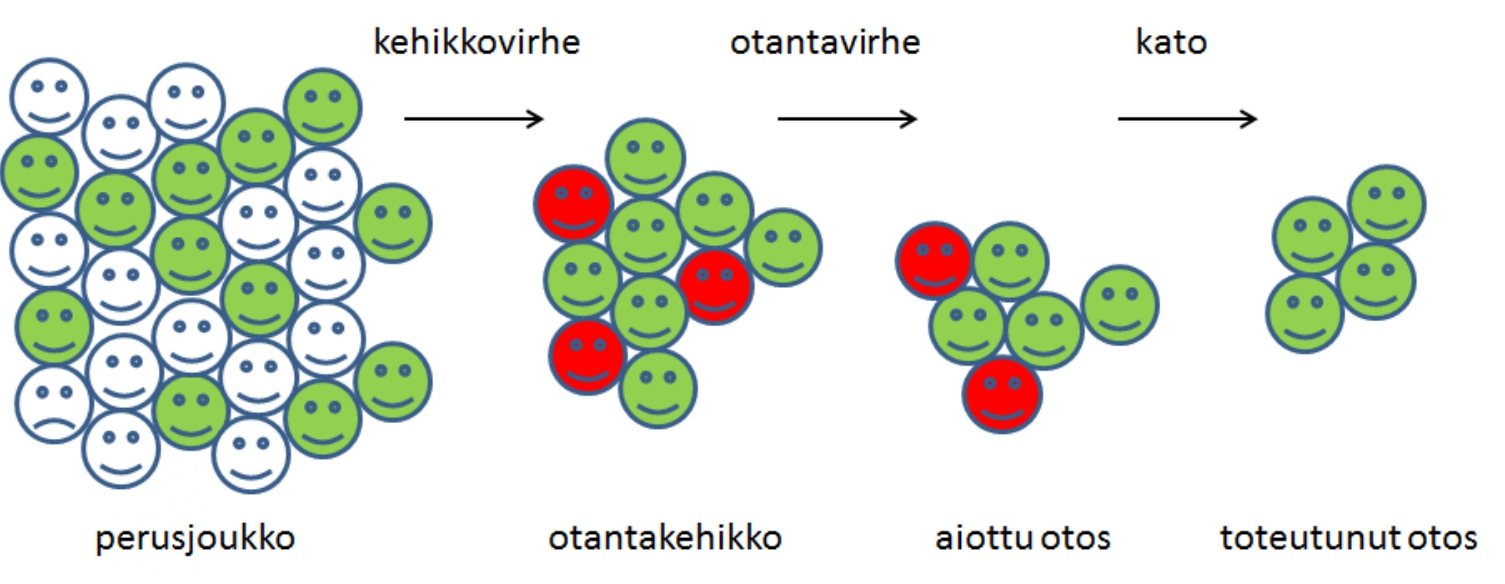
\includegraphics[width=1\linewidth]{images/otanta} 

}

\caption{Otannan idea.}\label{fig:otanta}
\end{figure}

\begin{itemize}
\tightlist
\item
  Edustavan otoksen avulla on mahdollista tehdä perusjoukkoa koskevaa tilastollista päättelyä, sillä otos kuvaa perusjoukon ominaisuuksia riittävän hyvin. Tämä on yksi tilastotieteen keskeisimpiä oppeja mutta myös kriittisen tiedelukutaidon ja arkijärjen kannalta tärkeää.
\end{itemize}

\begin{eblock}{}

\textbf{Esimerkki: Kotitalouksien tulot, tuloerot ja pienituloisuusrajan kehitys 1987-2005 (Tilastokeskus)}

\begin{itemize}
\tightlist
\item
  Tilastotyksikkö kotitalous, joten kaikkien kotitalouksien tutkiminen (kokonaistutkimus, ks. alla) olisi vaikeaa ja aikaavievää.
\item
  Tutkittavaksi valitaan vain muutama tuhat kotitaloutta (ts. otantatutkimus) ja selvitetään näiden tulot.
\item
  On mahdollista tehdä \textbf{kaikkia} suomalaisia kotitalouksia koskevia johtopäätöksiä, jos tutkitut yksiköt olivat \textbf{edustava otos} suomalaisista kotitalouksista. Ts. osajoukkoa koskevat päätelmät voidaan yleistää koskemaan perusjoukkoa, mikäli osajoukko on edustava otos perusjoukosta.
\end{itemize}

\end{eblock}

\begin{figure}

{\centering 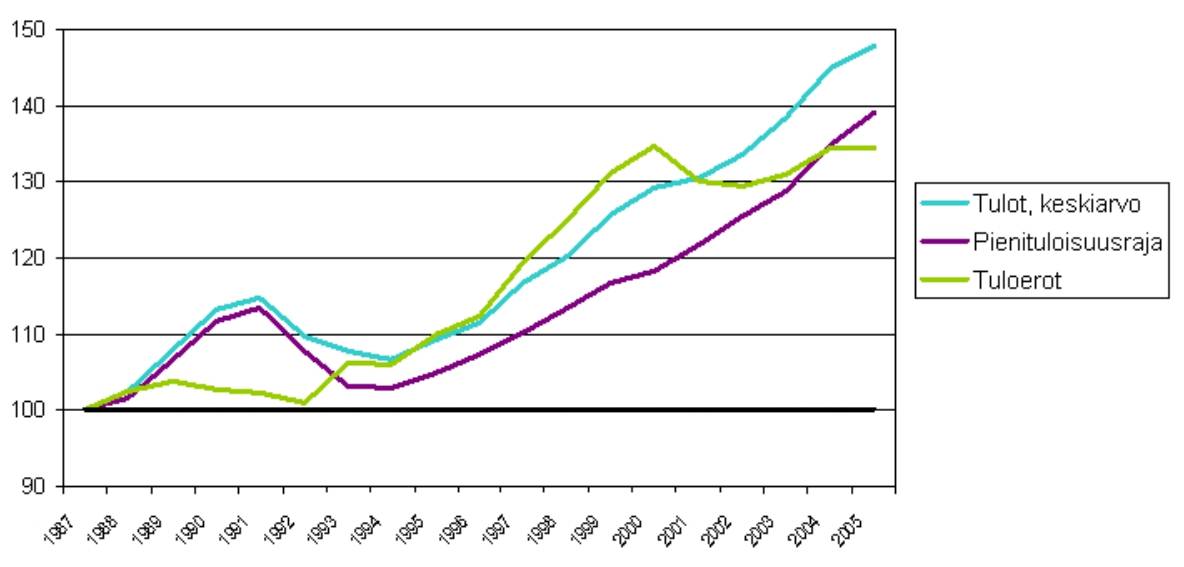
\includegraphics[width=1\linewidth]{images/tuloerot} 

}

\caption{Tuloerot.}\label{fig:tuloerot}
\end{figure}

\hypertarget{alaluku53}{%
\subsection{Tilastollisten muuttujien mittaaminen ja mitta-asteikot}\label{alaluku53}}

\textbf{Mittaaminen}

\begin{itemize}
\item
  Tilastotieteellinen tutkimus perustuu aina mitattaviin satunnaisilmiöihin: tavoitteena on mittaamalla liittää jokin luku ilmiötä kuvaavaan ominaisuuteen, ts. mitata kyseisen satunnaismuuttujan havaittua arvoa.
\item
  Kumpaa tahansa tutkimusotetta (kokonais- tai otantatutkimus) noudatettaessa tietojen keräämisessä on olennaisena osana kohteiden ominaisuuksien \textbf{mittaaminen}.

  \begin{itemize}
  \tightlist
  \item
    Mittaaminen vaatii aina mittauksen kohteen, hyvin määritellyn mitattavan ominaisuuden ja \textbf{mittarin}, joka liittää mielekkäät lukuarvot mitattavaan ominaisuuteen.
  \item
    Erilaiset mittarit heijastavat ilmiön ominaisuuksia eri tavoin ja eri tarkkuudella

    \begin{itemize}
    \tightlist
    \item
      Esimerkiksi jos tutkitaan opiskelijoiden pituuden kehitystä niin mitataan pituutta eri aikoina. Pituudet voidaan mitata senttimetreissä, metreissä, kilometreissä tai vaikkapa tuumissa.
    \item
      Mittari on hyvä jos sen antama mittaus on

      \begin{itemize}
      \tightlist
      \item
        \textbf{(i) validi} eli mittaus esittää oikein mitattavaa ominaisuutta (senttimetri mittaa pituutta, gramma ei) ja
      \item
        \textbf{(ii) luotettava} eli mittaus on \textbf{harhaton} ja \textbf{toistettavissa}.
      \end{itemize}
    \item
      Määritellään nämä termit vielä erikseen, sillä ne ovat keskeisiä tilastotieteessä.
    \end{itemize}
  \end{itemize}
\end{itemize}

\begin{defblock}{}
\textbf{Harhattomuus}

Mittari on harhaton, jos se ei systemaattisesti ali- tai yliarvioi mitattavan ominaisuuden määrää.

\end{defblock}

\begin{itemize}
\item
  Harhaton mittari siis antaa keskimäärin oikeita mittauksia mitattavasta ominaisuudesta.
\item
  Harhattomuutta pidetään myös hyvänä ominaisuutena tilastollisten mallien parametrien estimaattoreille. Tähän palataan myöhemmin luvussa \ref{luku6}.
\end{itemize}

\begin{defblock}{}
\textbf{Toistettaavuus}

Mittari on toistettava, jos se tuottaa keskimäärin samanlaisia mittauksia samanlaisista otoksista eli se on johdonmukainen ja mittausvirheet ovat pieniä.

\end{defblock}

\begin{itemize}
\item
  Huonosti toistettava mittari antaa tilastoyksiköiden samankaltaisille ominaisuuksille hyvin erilaisia arvoja riippuen otoksesta.
\item
  \textbf{Mittausten reliabiliteettia/luotettavuutta} arvioidessa voidaan pohtia esimerkiksi seuraavia kysymyksiä:

  \begin{itemize}
  \tightlist
  \item
    Kuinka hyvin mittaustulokset ovat toistettavissa, kuinka paljon niissä on ei-sattumanvaraisuutta?
  \item
    Mittausten validiteetti: kuinka hyvin pystyttiin mittaamaan sitä, mitä oli tarkoitus mitata?
  \end{itemize}
\item
  Kun mittaaminen on luotettavaa ja validia, tutkimusaineisto on \textbf{sisäisesti luotettavaa}.
\item
  Aineiston \textbf{ulkoinen luotettavuus} toteutuu silloin, kun tutkittu otos edustaa perusjoukkoa eli on edustava. Validi mittaaminen ei pelasta epäedustavaa otosta!
\item
  Jokaisen tutkimuksen tulosten luotettavuuden perusteena on käytetty aineisto, kuinka se on hankittu ja mistä lähteestä. Kun käytetään luotettavaksi havaittuja mittareita, voidaan kustakin aineistosta laskea erikseen tunnuslukuja mittauksen luotettavuudelle. Esimerkkinä \textbf{luottamusväli}:

  \begin{itemize}
  \tightlist
  \item
    Luottamusväliä käytetään määrittämään estimaatin luotettavuutta.
  \item
    Väli, joka vaihtelee otoksesta toiseen ja joka usein sisältää mielenkiinnon kohteena olevan parametrin, kun otantakoetta toistetaan!
  \end{itemize}
\end{itemize}

\begin{figure}

{\centering 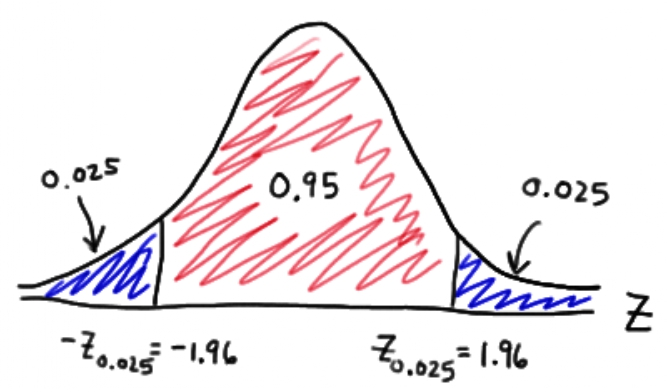
\includegraphics[width=1\linewidth]{images/luottamus} 

}

\caption{Normaalijakauman luottamusväli. Väliestimointia tarkastellaan tarkemmin seuraavassa luvussa.}\label{fig:luottamus}
\end{figure}

\begin{itemize}
\tightlist
\item
  Luotettavuudella voidaan tarkoittaa myös tutkimuksen \textbf{objektiivisuutta / puolueettomuutta}

  \begin{itemize}
  \tightlist
  \item
    \textbf{Objektiivinen totuus}, tutkimustulokset ovat samat riippumatta siitä kuka pätevä tutkija tutkimuksen on tehnyt.
  \item
    Tulosten tulisi olla luotettavia, mutta luotettavatkin havainnot voivat olla puolueellisia siinä mielessä, että ne tarkastelevat asiaa vain yhdeltä näkökannalta!
  \item
    Esim. tarkastellaan yrityksen henkilöstökysymyksiä, työn organisointia ja työmoraalia, ongelmien tarkastelu johdon vs.~henkilöstön näkökulmasta.
  \end{itemize}
\end{itemize}

\begin{eblock}{}

\textbf{Esimerkki: C-vitamiinin vaikutus syövän hoidossa}

\begin{itemize}
\item
  Annettiin C-vitamiinia 100 terminaalivaiheen syöpäpotilaalle ja
  seurattiin kuolleisuutta (Cameron and Pauling, 1976).

  \begin{itemize}
  \tightlist
  \item
    Pyrittiin luomaan tärkeiden ominaisuuksien suhteen samanlaisia verrokkiryhmiä ja valittiin kutakin potilasta kohden 10 verrokkia, jotka olivat samanlaisia iän, sukupuolen, primääri-kasvaimen sijaintipaikan ja histologisen kasvaintyypin suhteen.
  \item
    Seuranta-aika: aika hetkestä, jolloin todettiin tavanomaisten hoitojen olevan tehottomia, kuolinhetkeen saakka.
  \item
    Tulos: C-vitamiinia saaneet käsittelyryhmän potilaat elivät 4 kertaa kauemmin (p \(< 0.0001\)).
  \end{itemize}
\item
  Ristiriitaista evidenssiä saatiin tutkimuksessa, jossa vastaava tutkimusongelma, mutta toteutettu satunnaistettuna kokeena (Moertel et al.~1985).

  \begin{itemize}
  \tightlist
  \item
    Satunnaistettiin potilaat, joilla pitkälle edennyt paksunsuolen tai peräsuolen syöpä, C-vitamiinia saavien ja lumelääkettä saavien ryhmiin.
  \item
    Tulos: kontrolliryhmän potilaat elivät keskimäärin hieman pidempään, mutta ero ei merkitsevä.
  \end{itemize}
\item
  Mistä kahden tutkimuksen erot johtuivat? Huonolla tuurilla kaltaistetut verrokit erosivat käsittelyryhmän potilaista joillakin merkittävillä tavoilla, joita ei oltu mitattu! Miten kvantifioida ``huonoa tuuria''?
\item
  Tilastolliset menetelmät tekevät juuri tämän: ``Mikä on todennäköisyys, että havaittu tulos (tai sitä enemmän nollahypoteesista poikkeava tulos) olisi syntynyt vain sattumalta?''

  \begin{itemize}
  \tightlist
  \item
    Ilman satunnaistamista tuota kenties merkittävää ei-mitattua eroa ei pystytä varmuudella kontrolloimaan.
  \item
    Todellisuudessa ero johtui siitä, että ensin mainitun tutkimuksen kontrollit valittiin jo kuolleista syöpäpotilaista, eikä heihin liittynyt enää mitään satunnaisuutta!
  \end{itemize}
\end{itemize}

\end{eblock}

\hfill\break
\hfill\break
\_Mitta-asteikot\_\_

\begin{itemize}
\item
  Kuten satunnaismuuttujia koskeneessa luvussa \ref{luku4} opittiin, satunnaisilmiöillä on erilaisia tulosvaihtoehtoja jotka kantavat satunnaismuuttujien todennäköisyysjakaumia.

  \begin{itemize}
  \tightlist
  \item
    On syytä huomauttaa, että vaikka mitattava ilmiö ei olisikaan numeerinen, se voidaan aina ``koodata'' eli muuntaa numeeriseksi. Esimerkiksi perinteinen kaksiarvoinen mies-nainen -muuttujan tapauksessa voidaan käyttää tunnuksia 0 ja 1.
  \end{itemize}
\item
  Ilmiön luonteesta riippuen voidaan näille tulosvaihtoehdoille käyttää erilaisia \textbf{mitta-asteikkoja}.

  \begin{itemize}
  \tightlist
  \item
    \textbf{Laatueroasteikko/luokitteluasteikko} (nominaaliasteikko): Muuttujan mittaustaso on tällöin sellainen, että sen arvot voidaan luokittaa toisistaan eroaviin luokkiin. Ts. mihin luokkaan kohde kuuluu mitattavan ominaisuuden perusteella?

    \begin{itemize}
    \tightlist
    \item
      Tilastoyksiköt luokitellaan ennaltamääriteltyihin luokkiin. Luokkien järjestyksellä ei ole merkitystä.
    \item
      Kukin tilastoyksikkö kuuluu vain yhteen luokkaan. Tällöin kahdesta tilastoyksiköstä/havainnosta voidaan päätellä vain kuuluvatko ne saamaan luokkaan vai eivät.
    \item
      Emme pysty määrittelemään empiirisesti mielekästä järjestystä havaintoarvojen välillä.
    \item
      Esimerkkejä: Sukupuoli, veriryhmä tai kotikunta.
    \end{itemize}
  \item
    \textbf{Järjestysasteikko} (ordinaaliasteikko): Tällöin muuttujan arvot voidaan luokittelun lisäksi asettaa empiirisesti mielekkääseen järjestykseen. Tällöin siis mittauksen kohteella on ``enemmän mitattavaa ominaisuutta'' kuin jollakin toisella kohteella

    \begin{itemize}
    \tightlist
    \item
      Tilastoyksiköt luokitellaan ennalta määrättyihin luokkiin, joilla on yksikäsitteinen järjestys.
    \item
      Esimerkkejä: Sotilasarvo, sosiaaliryhmä, kilpailun tulos tai sairauksien tarttuvuus.
    \end{itemize}
  \item
    \textbf{Välimatka-asteikko} (intervalliasteikko): Luokittamisen ja järjestyksen asettamisen lisäksi havaintoarvojen välimatkalla on empiirisesti mielekäs tulkinta. Ts. intervalliasteikon tasoisen muuttujan arvoista voidaan sanoa, kuinka paljon toinen arvo on toista suurempi (pienempi).

    \begin{itemize}
    \tightlist
    \item
      Välimatka-asteikolla pystytään mittaamaan yksittäisten luokkien tai havaintoarvojen ero. Esimerkiksi: Lämpötilan mittaaminen esim. celcius-asteina. Pystymme numeroarvoina ilmoittamaan onko tänään lämpimämpi, yhtä lämmin vai kylmempi sää kuin eilen ja kuinka monta astetta muutos on.
    \item
      Kuinka paljon kahden mittauksen kohteen ominaisuudet eroavat toisistaan.
    \item
      Intervalliasteikon tasoisen muuttujan arvoista voidaan sanoa, kuinka paljon toinen arvo on toista suurempi (pienempi). Mittarin nollapiste on kuitenkin ``keinotekoinen'' ja siten vapaasti valittavissa. Samoin voidaan valita käytettävä mittayksikkö vapaasti. Oleellista on vain se, että havaintojen välisellä välimatkalla on aina empiirisesti mielekäs tulkinta.
    \item
      Yhteen- ja vähennyslasku ovat sallittuja.
    \end{itemize}
  \item
    \textbf{Suhdeasteikko}: Jos intervalliasteikon ominaisuuksien lisäksi on määriteltynä yksikäsitteinen mittalukujen absoluuttinen nollapiste.

    \begin{itemize}
    \tightlist
    \item
      Esimerkiksi kuuden euron hintainen tuote on kaksi kertaa niin kallis kuin kolmen euron tuote.
    \item
      Kunnan veroäyri tai henkilön pituus: Absoluuttinen nollapiste on 0.
    \item
      Nollapisteen ollessa absoluuttinen, se ``pysyy paikallaan'' ja mittalukujen suhteet pysyvät samoina.
    \end{itemize}
  \end{itemize}
\item
  Mitta-asteikot voidaan jakaa kahteen luokkaan: \textbf{Luokittelu- ja järjestysasteikkoa kutsutaan kvalitatiivisiksi asteikoiksi}. Tällöin muuttujien arvot kuvaavat vain tilastoyksiköiden laadullisia piirteitä.
\item
  Vastavasti \textbf{välimatka- ja suhdeasteikkoa kutsutaan kvantitatiivisiksi asteikoiksi}, koska tällöin mittaluvut kuvaavat jonkin ominaisuuden määrää.
\item
  Tilastollisen analyysin kannalta mitta-asteikkojen merkitys on siinä, että tilastollisten (matemaattisten) operaatioiden sallittavuus määräytyy muuttujan mitta-asteikon mukaan. Mitä korkeampi mitta-asteikko, sitä enemmän on käytettävissä olevia analyysimenetelmiä. Esimerkiksi keskiarvon laskeminen on eräs tilastollinen operaatio, ja se ei ole sallittu kvalitatiivislle muuttujille.
\item
  \textbf{Aineistotyyppejä}: Käsitellään tarkemmin vielä myöhemmin (Luvussa \ref{luku10}), joiden yhteydessä mitattavat muuttujat voivat olla kvalitatiivisia tai kvantitatiivisia.

  \begin{itemize}
  \tightlist
  \item
    Poikkileikkausaineisto: Tietoja yhdeltä ajanhetkeltä tai aikaväliltä
  \item
    Aikasarja-aineisto: Tietoja samasta tutkimuskohteesta eri ajanhetkiltä
  \item
    Paneeliaineisto: Tietoja useilta ajanhetkiltä useista tutkimuskohteista
  \item
    Tapahtumahistoria-aineisto: Tietoja tapahtumahetkiltä
  \end{itemize}
\end{itemize}

\hypertarget{alaluku54}{%
\subsection{Kontrolloidut kokeet ja suorat havainnot}\label{alaluku54}}

\begin{itemize}
\item
  Tilastollinen tutkimusaineisto voidaan kerätä:

  \begin{itemize}
  \tightlist
  \item
    \textbf{Kontrolloiduilla kokeilla}, joissa tutkimuksen kohteet altistetaan suunnitelmallisesti erilaisiin koeolosuhteisiin selvittääkseen miten kohteet reagoivat muutoksiin.
  \item
    \textbf{Suoria havaintoja} tehtäessä koeolosuhteita ei pyritä aktiivisesti muuttamaan vaan ainoastaan seurataan miten erilaiset olosuhteet ja niissä tapahtuvat muutokset vaikuttavat kohteisiin.
  \end{itemize}
\item
  Näistä tutkimusasetelmista kontrolloidut kokeet ovat tietenkin ihanteellisempia tutkimuksen tekemiselle, sillä tutkijan on mahdollista tarkastella tutkittavaa asiaa koeolosuhteissa ``eristyksissä''.
\item
  Kontrolloidut kokeet eivät kuitenkaan ole aina mahdollisia, jolloin on käytettävä suoria havaintoja.

  \begin{itemize}
  \tightlist
  \item
    Tällöin tutkimuskohdetta ei suunnitelmallisesti altisteta koeolosuhteille (``käsittelyille'') vaan muuttuvien olosuhteiden vaikutuksia tilastoyksikköihin seurataan passiivisesti.
  \item
    Toisin sanoen tutkimuksen kohteena olevat tilastoyksiksöt eivät välttämättä edes tiedä osallistuvansa tutkimukseen.
  \end{itemize}
\item
  Lisäksi usein tehdään hoito/käsittelyvastetta koskevia vertailuja erilaisissa olosuhteissa, joka osaltaan vaikuttaa tulosten uskottavuuteen, sillä tutkittaviin tilastoyksiköihin voi vaikuttaa olosuhteiden muutosten lisäksi muut ulkopuoliset tekijät.

  \begin{itemize}
  \tightlist
  \item
    Näiden \textbf{selittävien} ja \textbf{sekoittavien tekijöiden} vaikutusten kontrollointi on suoria havaintoja tehtäessä vaativa tehtävä.
  \item
    Mikäli ulkopuolisia tekijöitä ei havaita ja/tai pystytä mittaamaan, tai muuten jostain syystä olla lisätty ja käytetty käytettävässä tilastollisessa mallissa, voi kyseeseen tulla ns. \textbf{puuttuvien selittäjien harha}, joka tarkoittaa sitä että havaittuihin tuloksiin vaikuttaa jokin havaitsematon tekijä, mutta jonka vaikutusta ei kyetä kvantifioimaan puutteellisten havaintoarvojen vuoksi.
  \end{itemize}
\item
  Suoria havaintoja tehtäessä ei voida (usein) selvittää vasteen ja olosuhteiden \textbf{kausaalista} yhteyttä. Suorilla havainnoilla voidaan lähinnä saada selville onko vasteella ja olosuhteilla jokin yhteys (korrelaatio) (ks. luku \ref{luku7}).
\item
  Suorien havaintojen keräämiseen liittyy olennaisesti joitain riskejä ja toisaalta rajoituksia. Riskit liittyvät käytännössä otoksen harhaisuuteen (erit. valikoitumisharha)

  \begin{itemize}
  \tightlist
  \item
    Esimerkiksi jos havaintoja tehtäessä suositaan systemaattisesti joitakin tulosvaihtoehtoja. Tämä suosiminen voi olla tahallista tai tahatonta.
  \item
    Tämä tilastoyksiköiden \textbf{valikoituminen} otokseen aiheuttaa harhaa, sillä otokseen valikoituva osajoukko saattaa ylikorostaa perusjoukon jotain ominaisuuksia.
  \end{itemize}
\end{itemize}

\begin{defblock}{}

\textbf{Valikoituminen}

Valikoitumista tapahtuu, jos otokseen poiminta ei ole riippumatonta tilastoyksikön ominaisuuksista. Tätä kutsutaan valikoitumisharhaksi.

\begin{itemize}
\item
  Esimerkiksi verrattaessa sydän- ja verisuonitautipotilaiden hoitotoimenpiteitä potilaat eivät mahdollisesti ole valikoituneet yhtä todennäköisesti pallolaajennukseen, ohitusleikkaukseen tai lääkehoitoryhmään, sillä taudin vakavuus saattaa jo määritellä mikä hoitotoimenpide valitaan.
\item
  Valikoituminen on iso ongelma seurantatutkimuksissa, sillä harhaisten havaintotulosten, eli harhaisen otoksen, perusteella ei voida tehdä luotettavia johtopäätöksiä perusjoukosta!
\end{itemize}

\end{defblock}

\begin{itemize}
\tightlist
\item
  Harhan syntymistä pyritään välttämään valitsemalla havaintojen kohteet perusjoukosta satunnaisesti (ellei tavoitteena ole tutkia kaikkia perusjoukon alkioita). Tämä merkitsee satunnaisotannan soveltamista havaintojen kohteiden valintaan, eli otokseen poimittavien tilastoyksiköiden valintaan sovelletaan \textbf{satunnaistamista}, jolloin sattuma määrää mitkä perusjoukon alkioista tulevat poimituksi otokseen (tutkimuksen kohteiksi)!
\end{itemize}

\begin{defblock}{}

\textbf{Satunnaistaminen}

Tilastoyksiköiden poimimista populaatiosta otokseen riippumatta muiden yksiköiden poiminnasta tai kyseisten (poimittavien) yksiköiden ominaisuuksista.

\begin{itemize}
\item
  Satunnaistaminen takaa sen, että mahdolliset sekoittavat tekijät ovat jakaantuneet tasaisesti tutkittavassa joukossa. Tällöin sekoittavat tekijät eivät aiheuta harhaa otokseen ja tutkimuksen tulokset voidaan yleistää koko populaatioon.
\item
  Satunnaistaminen poistaa otannasta valikoitumisharhan, sillä otokseen poiminta suoritetaan riippumatta tilastoyksiköiden ominaisuuksista. Satunnaistaminen on ainoa puolueeton tapa poimia otos (ei suosi mitään perusjoukon osaa)!
\end{itemize}

\end{defblock}

\begin{itemize}
\item
  Satunnaistaminen (osaltaan) mahdollistaa \textbf{tilastollisen päättelyn}, jonka avulla otoksesta saatuja tietoja voidaan hyödyntää tehtäessä päätelmiä koko perusjoukosta.

  \begin{itemize}
  \tightlist
  \item
    Tilastollisen päättelyn avulla voidaan muodostaa esimerkiksi jakaumien ja tilastollisten mallien tuntemattomille parametreille arviot (piste-estimaatit) ja arvioida niiden epävarmuutta (keskivirheet ja luottamusvälit) sekä testata tarkasteltavaan ilmiöön liittyviä hypoteeseja (ks. luku \ref{luku6} ).
  \end{itemize}
\item
  Johtopäätelmien pätevyys riippuu mm. siitä, kuinka hyvin otanta on suoritettu. Tämän vuoksi on tärkeää ymmärtää otannan perusperiaatteet ja erilaisten otantamenetelmien luonne.
\item
  Kontrolloiduissa kokeissa satunnaistaminen jakaa yksilöt \textbf{riippumatta yksilön omista ilmiöön vaikuttavista muuttujista} joko \textbf{käsittely- tai kontrolliryhmään} (eng. treatment ja control).

  \begin{itemize}
  \tightlist
  \item
    Se takaa, ettei valikoitumista jonkin käsittelyä edeltävän ominaisuuden mukaan esiinny
  \item
    Tämä tarkoittaa \textbf{altisteen} (käsittely / ``treatment'\,') antamista (täysin) satunnaisesti kokeeseen valituille yksilöille, riippumatta näiden taustamuuttujien arvoista.
  \item
    Nämä yksilöt sinänsä voivat olla satunnaisotos jostain populaatiosta (tai ainakin niiden toivotaan olevan), mutta satunnaistaminen tarkoittaa siis käsittelyn kohdentamista koeyksilöille, ei satunnaisotantaa sinänsä
  \item
    Esimerkiksi tutkittavat voidaan satunnaistaa lääkehoito- ja placeboryhmiin, jotta mahdolliset erot tutkittavien iässä, sukupuolessa ja muissa taustamuuttujissa eivät aiheuta systemaattista harhaa, kun tutkitaan lääkehoidon vaikutusta.
  \end{itemize}
\end{itemize}

\hypertarget{alaluku55}{%
\subsection{Otantamenetelmät}\label{alaluku55}}

\begin{itemize}
\tightlist
\item
  Tässä jaksossa tarkastellaan erilaisia \textbf{otantamenetelmiä}. Näiden menetelmien tarkoitus on suorittaa otosaineiston (tutkimusaineiston) kerääminen niin, että se huomioi aiemmin esitellyt hyvän otannan kriteerit, ts. että sen tuottama otos on edustava ja luotettava. Näin ollen otos kuvaa koko perusjoukkoa.

  \begin{itemize}
  \tightlist
  \item
    Otantamenetelmän, joskus myös \textbf{otanta-asetelman}, valinta on tietenkin vahvasti sovellusalakohtainen: käytettävät aineistot ja täten otantamenetelmät määräytyvät pitkälti tehtävän tutkimuksen luonteen perusteella. Ts. käytännön tilanteet poikkeavat toisistaan lopulta varsin paljon ja eri tilanteisiin tarvitaan omat menetelmänsä.
  \item
    Otanta-asetelmalla tarkoitetaan erityisesti otoksen poimintaan käytettyä \textbf{satunnaistuksen menetelmää}.
  \end{itemize}
\item
  Otannan tavoitteena on tietenkin edustava otos. Otoksen edustavuuteen vaikuttaa käytännön otannassa se, miten todennäköistä kullakin perusjoukon alkiolla (populaation tilastoyksiköllä) on tulla poimituksi otokseen. Tätä kutsutaan \textbf{sisältymistodennäköisyydeksi}.
\end{itemize}

\begin{defblock}{}
\textbf{Sisältymistodennäköisyys}

Sisältymistodennäköisyys kuvaa sitä (tunnettua) todennäköisyyttä, jolla perusjoukon alkio tulee poimituksi otokseen.

\end{defblock}

\begin{itemize}
\tightlist
\item
  Käytännössä otoksen poiminta suoritetaan niin, että \(n\):n alkion otos (\(n\) on otoskoko) poimitaan jollakin satunnaisotannan menetelmällä \(N\):n alkion perusjoukosta (\(N\) on siis perusjoukon koko).
\item
  Perusjoukon yksittäinen alkio (tilastoyksikkö) \(k\) tulee poimituksi \(n\):n alkion otokseen (tutkimusaineistoon) tunnetulla \textbf{sisältymistodennäköisyydellä} \(\pi_k\),
  \[
  0 < \pi_k \le 1, \quad k = 1, \ldots, N,
  \]
  jossa siis \(N\) on perusjoukon alkioiden lukumäärä. Toisin sanoen, kaikilla perusjoukon alkioilla on oma nollaa suurempi todennäköisyytensä (voi olla 1), \(\pi_k\), tulla poimituksi otokseen.

  \begin{itemize}
  \tightlist
  \item
    Sisältymistodennäköisyys voi olla sama kaikille perusjoukon alkioille tai vaihdella perusjoukon eri osajoukkojen (alkioryhmien) välillä. Tämä tulee huomioida otantamenetelmän valinnassa, jotta saadun otoksen edustavuus ei vaarannu.
  \item
    Sisältymistodennäköisyyttä voidaan käyttää monimutkaisemmassa otantateoriassa \textbf{asetelma}- ja \textbf{analyysipainojen} muodostamisessa sekä uudelleenpainotuksessa (vastauskadon korjaus).
  \end{itemize}
\item
  Tässä luvussa käsitellään erilaisia perinteisiä otantamenetelmiä sekä sitä, minkälaisten perusjoukkojen tilanteissa mikäkin otantamenetelmä on sopivin.

  \begin{itemize}
  \tightlist
  \item
    \textbf{Yksinkertainen satunnaisotanta} (YSO): perinteisin otantamenetelmä, jossa jokaisella tietyn kokoisella otoksella sama mahdollisuus tulla valituksi.
  \item
    \textbf{Systemaattinen otanta} (SYS):
  \item
    \textbf{Ositettu otanta}: perusjoukko (populaatio) jaetaan ominaisuuksiltaan yhtenäisiin eli homogeenisiin \textbf{ositteisiin}, joista jokaisesta poimitaan erillinen otos.
  \item
    \textbf{Ryväsotanta} tai joskus myös \textbf{moniasteinen otanta}: Hyödynnetään perusjoukossa esiintyvää kerroksellisuutta, eli hierarkkisuutta otannassa.
  \end{itemize}
\end{itemize}

\hypertarget{yksinkertainen-satunnaisotanta}{%
\subsubsection{Yksinkertainen satunnaisotanta}\label{yksinkertainen-satunnaisotanta}}

\begin{itemize}
\tightlist
\item
  \textbf{Yksinkertaisessa satunnaisotannassa} (YSO) jokaisella tilastoyksiköllä (perusjoukon alkiolla) on nollasta poikkeava todennäköisyys tulla valituksi otokseen.

  \begin{itemize}
  \tightlist
  \item
    Otanna satunnaisuus tulee siis siitä, että jokainen tilastoyksikkö poimitaan otokseen \emph{satunnaisesti}! (Ks. luku \ref{luku4})
  \item
    YSOa pidetään otannan perusmuotona, jossa jokaisella perusjoukon alkiolla on lähtökohtaisesti yhtä suuri todennäköisyys tulla valituksi otokseen.

    \begin{itemize}
    \tightlist
    \item
      Yksinkertainen satunnaisotanta on periaatteiltaan intuitiivinen ja helppo ymmärtää. Lisäksi se on tietyissä tilanteissa usein helppo toteuttaa.
    \end{itemize}
  \item
    Tällöin on selvää että myös jokaisella perusjoukon samankokoisella osajoukolla on sama todennäköisyys tulla valituksi.
  \item
    Toisin sanoen, todennäköisyys tulla poimituksi ei riipu tilastoyksikön ominaisuuksista tai siitä minkälaisia ominaisuuksia jo poimituilla otosyksiköillä on.
  \item
    Satunnaisotanta siis selvästi korjaa valikoitumisharhaa (viittaus aiempaan lukuun) satunnaistamalla otokseen valikoitumisen täysin! YSO voidaankin aina tulkita arvonnaksi. Käytännön työssä arvonta onkin oiva satunnaistamisen keino.
  \end{itemize}
\item
  \textbf{YSO:n toteuttaminen}

  \begin{itemize}
  \tightlist
  \item
    Käytännössä yksinkertainen satunnaisotanta etenee vaiheittain:

    \begin{itemize}
    \tightlist
    \item
      Tutkimuksen alussa tutkijalla tulisi olla käytettävänään (ts. tulisi koostaa) lista kaikista perusjoukon havaintoyksiköistä (alkioista). Tämä muodostaa tutkimuksen \textbf{otantakehikon}.
    \item
      Tämän jälkeen jokaiseen perusjoukon alkioon voidaan liittää numeeriset tunnukset.
    \item
      Sitten valitaan haluttu otoksen koko. Otoskoon määrittäminen on keskeinen osa koesuunnittelua, ks. luku \ref{alaluku66}
    \item
      Otantakehikosta arvotaan perusjoukon alkiot otokseen yksi kerrallaan.
    \item
      Käytännössä arvonta voidaan toteuttaa satunnaislukuja generoimalla (tuottamalla) niin että jokaisen otantakehikon alkion sisältymistodennäköisyys on yhtä suuri.\footnote{Satunnaislukujen generointia käsitellään ja opetellaan mm. R-kurssilla ja kurssilla \href{https://opas.peppi.utu.fi/fi/opintojakso/TILM3705/92210}{TILM3705 Johdatus laskennalliseen tilastotieteeseen.}}
    \end{itemize}
  \end{itemize}
\item
  YSO:n \textbf{poimintastrategiat}: Käytännössä yksinkertainen satunnaisotanta voidaan suorittaa kahdella eri tavalla: \textbf{palauttaen} tai \textbf{palauttamatta}.

  \begin{itemize}
  \tightlist
  \item
    Tarkastellaan, aiemman mukaisesti, \textbf{äärellistä populaatiota} (perusjoukkoa), jossa on \(N\) alkiota ja tarkoituksena on poimia \(n\):n alkion kokoinen otos (huom. \(n<N\)). Olkoon \(i\) yksittäisen alkion indeksiluku (ts. jokainen alkio on numeroitu esimerkiksi tavalla \(i = 1,\ldots,N\)).
  \end{itemize}
\end{itemize}

\textbf{YSO:n poiminta palauttaen}

\begin{itemize}
\tightlist
\item
  Kun poiminta suoritetaan \textbf{palauttaen}, niin poimittu alkio palautetaan aina ennen uuden alkion arpomista takaisin perusjoukkoon, jolloin alkio voi tulla poimituksi otokseen useita kertoja.

  \begin{itemize}
  \tightlist
  \item
    Kyseessä on siis otanta \textbf{takaisinpanolla} (with replacement).
  \item
    Tällöin alkioiden arvonnat ovat riippumattomia: alkion todennäköisyys tulla poimituksi otokseen ei riipu siitä kuinka monta alkiota otokseen on jo poimittu.
  \item
    Alkion \(i\) sisältymistodennäköisyys on tällöin selvästi
  \end{itemize}
\end{itemize}

\[
\pi_i = \frac{1}{N}, \quad \forall \, i
\]

\begin{itemize}
\item
  Otantaan palauttaen liittyviä todennäköisyyksiä hallitaan \textbf{binomijakauman} avulla (ks. luku 4), joka johtaa yksinkertaiseen \textbf{tilastolliseen malliin} YSO:a käytettäessä.
\item
  Poiminta palauttaen, tai otanta takaisinpanolla, on toisaalta varsin epärealistinen otantamenetelmä useassa tutkimuksessa. Esimerkiksi lienee mahdotonta testata samaa lääkettä useaan otteeseen samaan aikaan yhdellä koehenkilöllä.
\end{itemize}

\textbf{YSO:n poiminta palauttamatta}

\begin{itemize}
\tightlist
\item
  Kun poiminta suoritetaan \textbf{palauttamatta}, poimittua alkiota ei palauteta perusjoukkoon poiminnan jälkeen eikä se täten voi tulla poimituksi otokseen kuin kerran.

  \begin{itemize}
  \tightlist
  \item
    Kyseessä on siis otanta \textbf{ilman takaisinpanoa} (without replacement).
  \item
    Tällöin alkioiden arvonnat eivät enää ole riipumattomia: alkion todennäköisyys tulla poimituksi otokseen riippuu siitä kuinka monta alkiota otokseen on jo poimittu.
  \item
    Alkion \(i\) sisältymistodennäköisyys on tällöin vastaavasti
  \end{itemize}
\end{itemize}

\[
\pi_i = \frac{1}{N - A_i},
\]

\begin{itemize}
\tightlist
\item
  Tässä \(A_i\) on jo poimittujen alkioiden lukumäärä ennen kyseistä \textbf{otositeraatiota}: ensimmäisen poiminnan kohdalla \(A_i = 0\), toisen kohdalla \(A_i = 1\) ja niin edespäin.

  \begin{itemize}
  \tightlist
  \item
    Ilman takaisinpanoa populaatiosta voidaan poimia \({N \choose n}\) erilaista otosta.\footnote{Kun otosyksiköiden järjestyksellä ei ole merkitystä. \({N \choose n}\) on ns. binomikerroin, joka saadaan kaavasta \({N \choose n} = \frac{N!}{n!(N-n)!},\) jossa \(N! = N \cdot (N-1) \cdot (N-2) \cdots 1\) on \(N\):n kertoma.}
  \item
    Otantaan palauttamatta liittyviä todennäköisyyksiä hallitaan \textbf{hypergeometrisen jakauman} avulla, joka johtaa (melko) yksinkertaiseen \textbf{tilastolliseen malliin} YSO:a käytettäessä.
  \end{itemize}
\end{itemize}

\begin{eblock}{}

\textbf{Esimerkki: Yksinkertaisen satunnaisotannan poimintastrategiat}

\begin{itemize}
\tightlist
\item
  Esimerkki: Poimitaan palloja kulhosta satunnaisesti.

  \begin{itemize}
  \tightlist
  \item
    Jos yksittäinen pallo (alkio) voi tulla poimituksi useammin kuin kerran, eli pallo palautetaan kulhoon sen poiminnan jälkeen, on kyseessä yksinkertainen satunnaisotanta takaisinpanolla.
  \item
    Vastaavasti jos pallo voi tulla valituksi vain kerran, eli pallo poistetaan kulhosta sen poiminnan jälkeen, on kyseessä otanta ilman takaisinpanoa.
  \end{itemize}
\end{itemize}

\end{eblock}

\textbf{Otoskoon vaikutus YSO:n}

\begin{itemize}
\tightlist
\item
  Yksinkertaisen satunnaisotannan erot takaisinpanolla ja ilman takaisinpanoa riippuvat otantakehikon (tai yleisemmin perusjoukon) koosta. Mikäli poimittava otos muodostaa suuren osan perusjoukosta (ts. \(\frac{n}{N}\) on ``suuri'', eli lähellä yhtä) menetelmät poikkeavat olennaisesti.
\item
  Toisaalta, jos perusjoukko on ääretön niin menetelmillä ei ole käytännössä eroa (ts. kun \(N \longrightarrow \infty\) niin \(\frac{n}{N} \longrightarrow 0\) eli todennäköisyys että sama alkio poimittaisiin otokseen useammin kuin kerran lähestyy nollaa otoskoon lähestyessä ääretöntä).

  \begin{itemize}
  \tightlist
  \item
    Monesti onkin (teoreettiselta) kannalta järkevää olettaa että otos poimitaan äärettömästä perusjoukosta vaikka perusjoukko tosiasiallisesti olisikin äärellinen (mutta riittävän ``iso'').
  \item
    Tällöin voidaan olettaa käytettävän otantaa takaisinpanolla, sillä siinä käytettävät tilastolliset mallit ovat yksinkertaisempia kuin otannassa ilman takaisinpanoa ja tämä helpottaa tilastollisessa päättelyssä käytettäviä kaavoja.
  \end{itemize}
\end{itemize}

\_YSO: Potentiaaliset ongelmat\_\_

\begin{itemize}
\tightlist
\item
  Monissa tapauksissa ei kuitenkaan ole helppoa saada listaa kaikista perusjoukon havaintoyksiköistä (jolloin menetelmän käyttö on mahdotonta).
\item
  Kyselytutkimuksissa perusjoukko on usein suuri ja laajalle alueelle hajaantunut. Henkilökohtaisten, kasvotusten toteutettavien, haastattelujen tekeminen vaatisi suuria resursseja (haastattelijat joutuisivat esim. matkustamaan ympäri Suomea satunnaisotokseen valikoituneiden henkilöiden asuinpaikkojen mukaan).
\item
  Tällaisissa tutkimustilanteissa käytetäänkin usein muunlaisia otantamenetelmiä.
\end{itemize}

\hypertarget{systemaattinen-otanta}{%
\subsubsection{Systemaattinen otanta}\label{systemaattinen-otanta}}

\begin{itemize}
\tightlist
\item
  Systemaattisessa, eli tasavälisessä, otannassa poimintakehikkoon (perusjoukkoon) kuuluvat alkiot järjestetään jonoon ja siitä poimitaan otokseen joka \(k\). alkio.

  \begin{itemize}
  \tightlist
  \item
    Esimerkiksi jos oletetaan että perusjoukkoon kuuluu 1000 tilastoyksikköä ja valittu otoskoko on 100, niin otos voidaan poimia perusjoukon alkioiden järjestetystä listasta poimimalla siitä joka kymmenes yksikkö.
  \item
    Systemaattinen otanta ei oikeastaan kuulu satunnaisotannaksi laskettaviin menetelmiin, koska siinä ei sovelleta arvontaa.
  \item
    Yksinkertainen satunnaisotanta voidaan kuitenkin nähdä systemaattisen otannan erikoistapauksena (eli systemaattinen otanta voidaan toteuttaa satunnaisotantana), missä perusjoukon alkiot järjestetään jonoon \textbf{satunnaistamalla}. - Ts. jonon järjestys on satunnainen, eli joka \(k\). jonon alkio on ``satunnaisotos'' otantakehikosta.
  \item
    Systemaattinen otanta tuottaa tällöin samat johtopäätelmät kuin yksinkertainen satunnaisotanta, jos perusjoukon alkioiden järjestys on tutkittavan ilmiön kannalta satunnainen! Toisin sanoen, harhaa ei synny mikäli perusjoukon alkioiden järjestys ei riipu sellaisesta ominaisuudesta, jota tutkitaan.
  \item
    Systemaattisen otannan suhteen potentiaaliseksi ongelmaksi muotoutuu havaintoyksikkölistan mahdollinen säännöllinen jaksollisuus, jota se ei havaitse ja jolloin satunnaisotanta toimisi (kenties) paremmin.

    \begin{itemize}
    \tightlist
    \item
      Ongelmia syntyy esimerkiksi silloin, jos tiedot perusjoukosta koostuvat pariskunnista ja poimintaintervalli on parillinen luku. Tällöin seurauksena voi olla, että otokseen saattaisi valikoitua ainoastaan joko miehiä tai naisia.
    \end{itemize}
  \end{itemize}
\item
  Myös systemaattisessa otannassa tarvitaan siis lista tai rekisteri kaikista perusjoukon havaintoyksiköistä ja sitä sovelletaankin tavallisesti YSO:n sijasta silloin, kun perusjoukon alkioista on käytettävissä tietorekisteri, luettelo tai havaintoja kerätään ajassa tai tilassa.

  \begin{itemize}
  \tightlist
  \item
    Esimerkiksi mielipidekyselyn kohteet poimitaan (voitiin poimia) puhelinluettelosta (tai vastaavasta rekisteristä) valitsemalla haastateltavaksi jokaiselta aukeamalta ensimmäisenä esiintyvä henkilö tai jotain tuotetta valmistavan tehtaan laaduvalvonnassa valitsemalla laatuarviointiin joka sadas tuote, joka hihnalta valmistuu. Muita esimerkkejä ovat esim. liikenteen, jäsenrekisteriin tai kassajonossa seisovien otantayksiköiden poiminta otokseen.
  \end{itemize}
\end{itemize}

\hypertarget{ositettu-otanta}{%
\subsubsection{Ositettu otanta}\label{ositettu-otanta}}

\begin{itemize}
\tightlist
\item
  Ositettu otanta on sopiva menetelmä tilanteisiin, joissa perusjoukko koostuu jonkin ominaisuuden suhteen homogeenisista ryhmistä, ts. alkioryhmistä (osista). Ositettu otanta pyrkii varmistamaan, että tutkittava otos on edustava kaikkien (tutkimuksen kannalta) olennaisten ryhmien osalta.

  \begin{itemize}
  \tightlist
  \item
    Esimerkiksi jos tavoitteena on tutkia jonkin maan erilaisten ja usein hyvin eri kokoisten kieliryhmien taloudellista asemaa. Kaikista ryhmistä tulisi saada edustava otos.
  \item
    Tällöin maan koko populaatioon kohdistettu yksinkertainen satunnaisotanta ei olisi järkevää, sillä otoskoon pitäisi olla (todennäköisesti) hyvin suuri, että jokaisesta kieliryhmästä saataisiin poimittua edustava otos.
  \item
    Ositetun otannan avulla otos voitaisiin kerätä niin, että jokaisesta ryhmästä (ositteesta) poimitaan osaotos yksinkertaisella satunnaisotannalla tai systemaattisella otannalla ja nämä osaotokset yhdistetään yhdeksi otokseksi.
  \end{itemize}
\item
  Ositettu otanta voi (oikein toteutettuna ja sopivassa asetelmassa) tuottaa paljon tarkempaa tietoa kuin yksinkertainen satunnaisotanta samaa otoskokoa käytettäessä! Voidaan esimerkiksi käyttää tietoa siitä, että otosyksiköt ovat joka ositteessa keskenään samankaltaisia.
\item
  Ositetun otannan käyttöön suurissa kyselytutkimuksissa liittyy samoja ongelma kuin yksinkertaiseen ja systemaattiseen satunnaisotantaan.

  \begin{itemize}
  \tightlist
  \item
    Otokseen valikoituneet vastaajat voivat olla mm. levittäytyneinä suurelle maantieteelliselle alueelle. Näin ollen otannan suorittaminen vaatii suuria kustannuksia.
  \item
    Onko (järkevä) osittaminen ylipäätään mahdollista toteuttaa tarkasteltavassa sovelluskohteessa?
  \end{itemize}
\end{itemize}

\hypertarget{ryvuxe4sotanta}{%
\subsubsection{Ryväsotanta}\label{ryvuxe4sotanta}}

\begin{itemize}
\item
  Ryväsotanta soveltuu tilanteisiin, joissa perusjoukko on ``ryvästeistä'' eli se voidaan jakaa luonnollisiin ryhmiin eli rypäisiin (eng. \emph{clusters}).
\item
  Rypäkset indikoivat aineiston luontaista hierarkkista, eli monitasoista- tai asteista rakennetta.

  \begin{itemize}
  \tightlist
  \item
    Esimerkkejä tällaisista ryhmistä ovat erilaiset yritykset tai koululuokat. Esimerkiksi yritykset muodostavat luonnollisesti eri ryppäitä, joiden alkiot ovat työntekijöitä ja koululuokat muodostavat koulun sisällä omia luonnollisia ryppäitään ja opiskelijat ovat alkioita näissä ryppäissä.
  \end{itemize}
\item
  Huomionarvoista onkin, että toisin kuin ositetussa otannassa, ryväsotannassa ryppäiden oletetaan olevan toistensa kanssa riittävän samankaltaisia, että jokaista rypästä ei tarvitse erikseen tutkia.

  \begin{itemize}
  \tightlist
  \item
    Tämä onkin yksi ryväsotannan tärkeimpiä motivointeja, sillä sitä usein perustellaan kustannustehokkuudella: sen sijaan että poimitaan satunnaisia koululaisia mahdollisesti suuresta määrästä kouluja, voidaan poimia satunnaisia ryppäitä (kouluja), joista tutkimusyksiköt eli koululaiset poimitaan.
  \item
    Lisäksi koulun sisällä koululuokat muodostavat aliryppäitä, joista voidaan edelleen poimia satunnaisotos, jotta päästään tutkimaan perusjoukon alkioita eli koululaisia esim. haastattelututkimuksen muodossa.
  \item
    Tavoitteena on vähentää tietojen keruun aiheuttamia kustannuksia samalla varmistaen, että otos on kuitenkin mahdollisimman edustava!
  \end{itemize}
\item
  Ryväsotannan voi suorittaa \textbf{yksi}- tai \textbf{kaksivaiheisena} ( \textbf{yksiasteinen/kaksiasteinen ryväsotanta} ).

  \begin{itemize}
  \tightlist
  \item
    \textbf{Kaksivaiheisessa ryväsotannassa}

    \begin{itemize}
    \tightlist
    \item
      \textbf{Ensimmäisessä vaiheessa} poimitaan joukko ryppäitä kaikkien ryppäiden joukosta, eli vain osa ryppäistä on mukana lopullisessa otoksessa.\\
    \item
      \textbf{Toisessa vaiheessa} poimitaan ensimmäisessä vaiheessa poimituista ryppäistä alkiotason otokset.
    \end{itemize}
  \item
    \textbf{Yksivaiheisessa ryväsotannassa} toisessa vaiheessa valitaan kaikki ensimmäisen vaiheen otosryppäiden alkiot, jolloin toisen vaiheen otanta typistyy ensimmäisen vaiheen ryppäiden alkioiden kokonaistutkimukseksi.
  \item
    Poiminnan eri vaiheissa voidaan soveltaa yksinkertaista satunnaisotantaa tai systemaattista otantaa.
  \end{itemize}
\item
  Ryväsotantaa käytetään usein suuria haastattelututkimuksia tehtäessä. Erityisesti, ryväsotantaa voidaan hyödyntää myös silloin, kun tutkijalla ei ole käytettävissään kattavaa listaa kaikista havaintoyksiköistä, mutta näiden muodostamat ryppäät on määritettävissä.
\item
  Ryväsotannan heikkoutena pidetään sitä, ettei aina ole helppoa muodostaa rypäitä, jotka ovat toistensa kaltaisia. Tulosten tarkkuus myös riippuu moninpaikoin siitä, kuinka hyvin rypäisiin jako onnistuu.
\end{itemize}

\begin{eblock}{}

\textbf{Esimerkkejä ryväsotannasta}

\begin{itemize}
\tightlist
\item
  Esimerkki 1:

  \begin{itemize}
  \tightlist
  \item
    Poimitaan oppilaitoksen opiskelijoista otos arpomalla ensin otos luokkahuoneista (=rypäistä).
  \item
    Arvotuissa luokkahuoneissa käydään sitten suorittamassa kysely.

    \begin{itemize}
    \tightlist
    \item
      Esim. Oppilaitoksen opiskelijoista voidaan poimia otos arpomalla ensin otos luokkahuoneista, jolloin luokkahuoneet ovat nk. ryppäitä.
    \item
      Mahdollisia ongelmia? Miten huomoida päivä- ja iltaopiskelijat? Tämän voisi toteuttaa arpomalla otos luokkahuoneista päiväsaikaan ja toinen otos ilta-aikaan. Tässä yhdistetään ryväsotantaan ositettu otanta, jolla taataan päivä- ja iltaopiskelijoiden edustus.
    \end{itemize}
  \end{itemize}
\item
  Esimerkki 2: Tutkittaessa tänä vuonna peruskoulun aloittavia voidaan ensin poimia otos kouluista, jolloin koulut ovat rypäitä. Tämän jälkeen arvotaan kustakin otokseen tulleesta koulusta tietty määrä tutkimuksen kohderyhmään kuuluvia oppilaita.
\end{itemize}

\end{eblock}

\hypertarget{alaluku56}{%
\subsection{Otantaesimerkkejä}\label{alaluku56}}

\begin{eblock}{}

\textbf{Esimerkki: Työllisyys ja työttömyys, Tilastokeskuksen työvoimatutkimus}

\begin{itemize}
\tightlist
\item
  Työvoimatutkimus on otostutkimus, jonka avulla tilastoidaan 15--74-vuotiaan väestön työmarkkinoille osallistumista, työllisyyttä, työttömyyttä ja työaikaa (yhden viikon aikana) kuukausittain, neljännesvuosittain ja vuosittain.

  \begin{itemize}
  \tightlist
  \item
    Työvoimatilastoja käytetään työvoimapoliittisten ennusteiden ja suunnitelmien laadinnassa, toimien seurannassa ja päätöksenteon tukena.
  \item
    Työmarkkina-aseman perusluokittelussa väestö jaetaan työllisiin, työttömiin ja työvoiman ulkopuolisiin.

    \begin{itemize}
    \tightlist
    \item
      Työlliset ja työttömät muodostavat työvoiman.
    \end{itemize}
  \item
    Työvoimatutkimuksen \textbf{perusjoukon} muodostavat Suomessa vakinaisesti asuvat 15--74-vuotiaat henkilöt.
  \item
    Työvoimatutkimuksen otos poimitaan \textbf{ositetulla satunnaisotannalla} väestön keskusrekisteriin perustuvasta Tilastokeskuksen väestötietokannasta kahdesti vuodessa.
  \end{itemize}
\item
  Ositetun satunnaisotoksen poiminta:

  \begin{itemize}
  \tightlist
  \item
    Tutkimus on paneelitutkimus, jossa samaa henkilöä haastatellaan viisi kertaa.
  \item
    Joka kuukauden otokseen kuuluu noin 12 000 henkilöä, keskimäärin noin joka 300. henkilö perusjoukosta.
  \item
    Yhden tutkimuskuukauden otos koostuu viidestä rotaatioryhmästä, jotka ovat tulleet tutkimukseen mukaan eri aikoina. Otos vaihtuu asteittain siten, että kolmena peräkkäisenä kuukautena vastaamisvuorossa ovat eri henkilöt.
  \end{itemize}
\item
  Julkisuudessa seurataan useimmiten kuukausittain työllisyyden ja työttömyyden muutoksia edellisen vuoden vastaavasta kuukaudesta. Vaihtoehtoisesti voidaan käyttää kausitasoitettuja lukuja, jolloin tilannetta voidaan verrata edelliseen kuukauteen.
\end{itemize}

\end{eblock}

\hfill\break
\hfill\break

\begin{eblock}{}

\textbf{Esimerkki: Terveys 2000}

\begin{itemize}
\tightlist
\item
  Terveys 2000 -tutkimuksen tavoite oli tuottaa ajankohtainen kattava kuva työikäisen ja iäkkään väestön terveydestä ja toimintakyvystä selvittämällä tärkeimpien terveysongelmien yleisyyttä ja syitä sekä niihin liittyvän hoidon, kuntoutuksen ja avun tarvetta.
\item
  Tutkimus koskee (koski) 18 vuotta täyttänyttä Suomen aikuisväestöä (perusjoukko), josta valitaan valtakunnallisesti edustava 10 000 henkilön otos.
\item
  Poimittiin kaksivaiheinen ryväsotos terveyskeskuspiireistä.

  \begin{itemize}
  \tightlist
  \item
    Ositus perustui yliopistosairaaloiden vastuualuiden väestömäärään suhteutettuun kiintiöintiin.
  \item
    Suurimmat 15 terveyskeskuspiiriä poimittiin otokseen ja lopuista 65:stä piiristä poimittiin loppuotos kussakin ositteessa systemaattisella (PPS) otannalla (sisältymistodennäköisyys suhteessa alkion kokoon).
  \end{itemize}
\end{itemize}

\end{eblock}

\hypertarget{alaluku57}{%
\subsection{Otannan haasteita vielä kootusti}\label{alaluku57}}

\begin{itemize}
\item
  Poimintaharha: Otos ei edusta populaatiota. Vaarana varsinkin silloin, kun otokseen tulleet populaation alkiot ovat valikoituneet tai ovat itse valinneet itsensä otokseen. Vastaavasti toisinaan otoksen peitto ei ole hyvä eli tällöin otanta ei kata koko perusjoukkoa tai se kattaa perusjoukon ja vähän muutakin.
\item
  Jos poimitaan tutkimukseen ne perusjoukon alkiot, jotka ovat tutkimuksen tekemishetkellä `saatavilla', niin kyseessä on \textbf{näyte}. Näyte ei siis kata ilmiön koko vaihtelua edustavan satunnaisotoksen tapaan.

  \begin{itemize}
  \tightlist
  \item
    Esimerkiksi perinteiset katukyselyt eivät ole hyvä otantatapa, sillä kadulla liikkujat eivät välttämättä kovin hyvin edusta tutkittavaa perusjoukkoa, ellei perusjoukkona ole kyseisellä kadulla kyseiseen aikaan liikkuvat ihmiset.
  \item
    Jos television ajankohtaisohjelma pyytää katsojia twiittaamaan mielipiteensä ajankohtaisesta asiasta, kyseessä on itse valikoituva näyte (osallistujat valitsevat itse itsensä).
  \end{itemize}
\item
  Vajaapeittävyys: Populaation alkioista ei ole välttämättä täydellistä luetteloa
\item
  Vastauskato: Tutkimuksen kohteita ei tavoiteta tai he kieltäytyvät vastaamatta. Kadon vuoksi lopullinen otoskoko saattaa jopa karsiutua pois tai jokin osajoukko on aliedustettuna.
\item
  Vastausharha: Kysymykset voivat olla huonosti muotoiltuja tai vastaajat voivat antaa vääriä tietoja.
\end{itemize}

\end{document}
